\chapter{Initial Verification of Quillen Models} \label{chap:quillen-rework}

\begin{frame}
\mode<article>{Model 3 from \cite{quillen2005} was solved with Abaqus 6.6, and the post-processing Excel macros were replaced with a Python program to extract \J values from an Abaqus log file and a MATLAB script to calculate and plot \hone \citep{renfro2009}.
Quillen's original models displayed much higher \hone values than expected at both the free surface and the symmetry plane.
The errors on the free surface and symmetry plane disappeared, as shown in \Cref{fig:quillen-rework-2009}, but the anomaly at the third node remained.
The results of additional development on these models follows.}
\mode<presentation>{\begin{columns}[c]\begin{column}{0.45\textwidth}
\begin{itemize}
\item Quillen model 3 solved with Abaqus 6.6
\item Model not modified
\item Anomalies at \(\phi=0, \frac{\pi}{2}\) disappeared
\item Anomaly at third node remained
\item Excel macros replaced with Python and MATLAB programs
\end{itemize}
\end{column}\begin{column}{0.45\textwidth}}
\begin{figure} \centering
\mode<article>{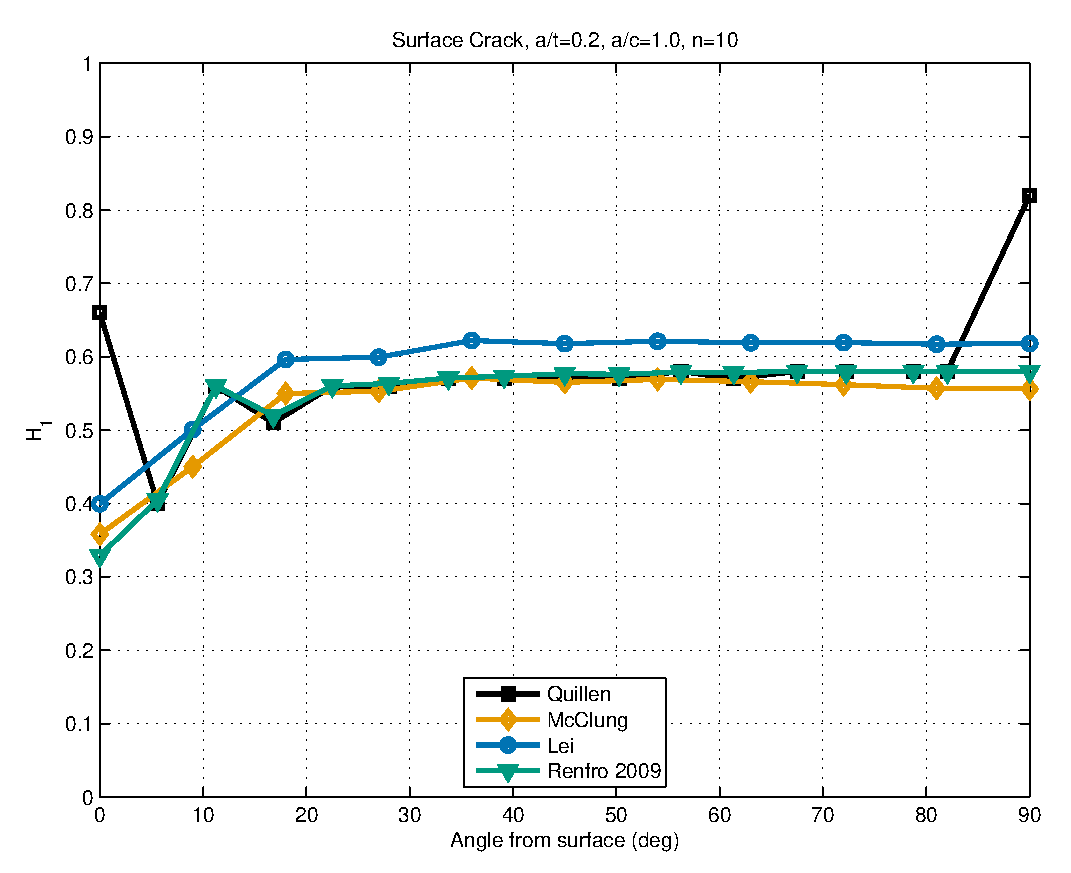
\includegraphics[width=\columnwidth]{model3_rework_2009}}
\mode<presentation>{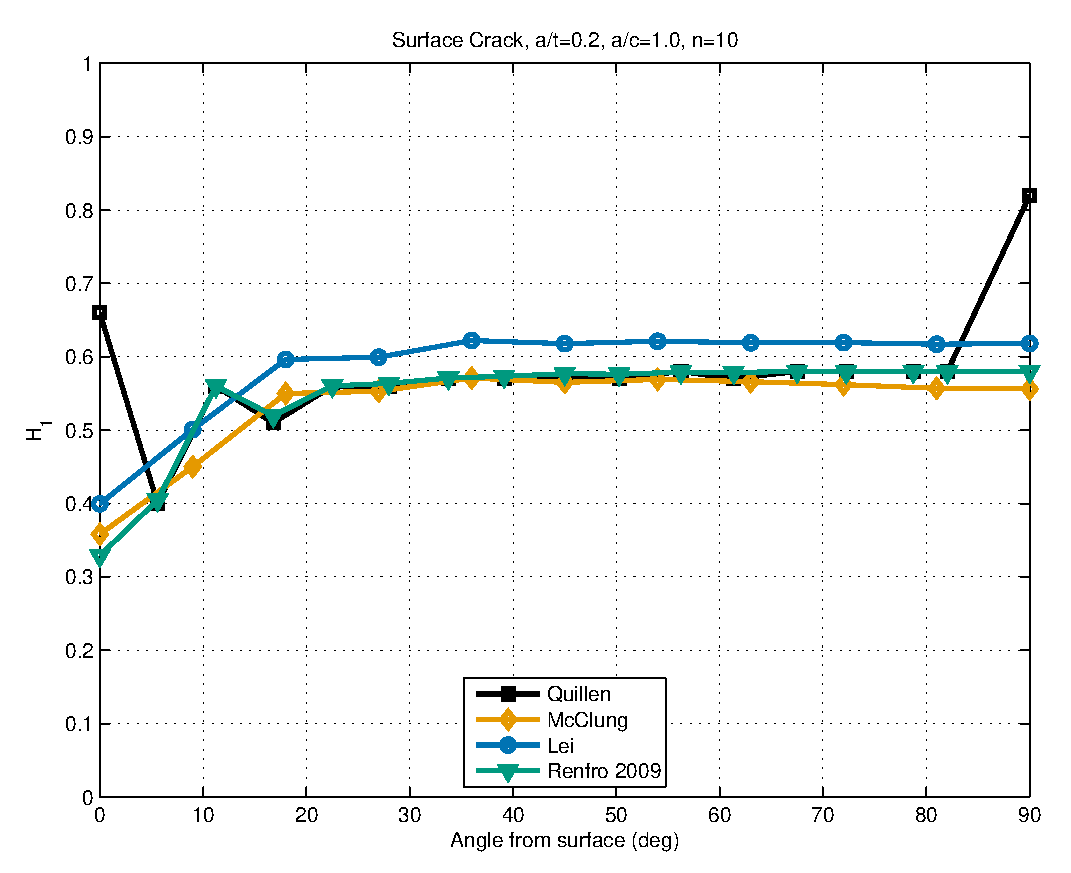
\includegraphics[width=\columnwidth]{model3_rework_2009}}
\mode<article>{\caption{\hone comparison between \citet{quillen2005} and \citet{renfro2009}, model 3, \(n=10\) \label{fig:quillen-rework-2009}}}
\end{figure}
\mode<presentation>{\end{column}\end{columns}}
\end{frame}
\note{In 2009, I ran one of Eric's models in a newer version of Abaqus with no modifications.

\vfill

Two of the three anomalies disappeared, but one remained.

\vfill

I converted his post-processing procedures from Excel macros to a more maintainable combination of Python and MATLAB.

\vfill
}

%\section{Development of Scripted Finite Element Models}

One disadvantage to the earlier finite element models is the difficulty in tracking changes to model input.
Most models are constructed interactively, which makes it difficult to isolate the critical differences between a working model and a non-working one.
Imagine having to click through every dialog box that could affect results, doing this on multiple models, and visually checking for differences in each of the material properties, boundary conditions, element types, etc.
In some cases, the user can write a plain-text file representing the model, but this can sometimes include lots of irrelevant information, or may simply contain a list of nodes and elements instead of driving variables such as mesh size parameters.

Details of the development of scripted finite element models are given in \Cref{chap:app-quillen-rework}, but the motivation can be summarized as a need to increase automation for parametric studies, to reduce opportunities for manual errors, to modularize and reduce duplicate code, and to improve tracking of changes made to models over time.
The resulting Python script was derived from an example given in the Abaqus~6.11-1 Benchmarks Manual \citeyearpar{abaqus-611-benchmarks-manual}, and can construct any of the tension models on demand, within a matter of seconds.

%Many finite element analysis software packages support the use of input files with a proprietary keyword syntax.
%Examples of this syntax include APDL (ANSYS parametric design language) and keyword syntax in Abaqus.
%Creating models with this method is more difficult for new users than with the graphical interactive method.
%However, since the keyword method is much closer to writing programs in a high-level programming language, it is much easier to isolate differences between models based off the differences in their input files.
%See \Cref{fig:material-apdl} for an example of a material property definition in APDL syntax, and \Cref{fig:material-abaqus-keyword} for the same material property definition in Abaqus keyword syntax.
%In both examples, the elastic modulus \(E\)\nomenclature[1E]{\(E\)}{elastic modulus} is defined on the first line, Poisson's ratio \(\nu\)\nomenclature[2\nu]{\(\nu\)}{Poisson's ratio} is defined on the second line, and both can be referenced wherever needed afterwards.
%
%\mode<presentation>{
%\begin{frame}
%\frametitle{Difficulty applying V\&V to finite element models}
%\begin{columns}[t]
%\begin{column}{0.45\textwidth}
%Most models
%\begin{itemize}
%\item constructed interactively in a GUI
%\item may require tedious verification of settings in every menu and dialog
%\item plain-text logs may exist
%\item logs may contain irrelevant information
%\item logs may omit critical parameters
%\end{itemize}
%\end{column}
%\begin{column}{0.45\textwidth}
%Some models
%\begin{itemize}
%\item constructed with proprietary input language
%\item allows some level of ``code verification''
%\end{itemize}
%\end{column}
%\end{columns}
%\end{frame}
%}
%\note{One thing that bothered me at the time, even though I didn't have a formal vocabulary for it, was that Eric's model was difficult to perform V\&V on.
%
%\vfill
%
%Most finite element models are like that---they're constructed interactively, with a GUI, and when (not if) errors or glitches happen, it's difficult to identify their origin.
%
%\vfill
%
%Some models (often simpler 2D ones) are constructed in an input language for the finite element program.
%
%\vfill
%
%This is an improvement in terms of code verification, but isn't always easily applied to more complex models.
%
%\vfill
%
%Eric's models were constructed in a third-party program (FEA-Crack) and analyzed in Abaqus.
%
%\vfill
%
%By 2009, we no longer had a license to FEA-Crack, and renewing it was prohibitively expensive.
%
%\vfill
%
%Though FEA-Crack used Abaqus' input language syntax, it basically wrote out a giant list of nodes and elements, making it difficult to impossible to determine why his models had anomalies at the third node.
%
%\vfill
%}
%
%\begin{frame}[containsverbatim]
%\begin{columns}[b]
%\begin{column}{0.5\textwidth}
%\begin{figure}
%\begin{lstlisting}[language={APDL}]
%! Define parameters
%E=30.0e6
%NU=0.3
%! Set material properties
%MP,EX,1,E
%MP,PRXY,1,NU
%\end{lstlisting}
%\caption{Material definition in APDL syntax \label{fig:material-apdl}}
%\end{figure}
%\end{column}
%\begin{column}{0.5\textwidth}
%\begin{figure}
%\begin{lstlisting}[language={Abaqus}]
%** Define parameters
%*PARAMETER
%E=30.0e6
%NU=0.3
%** Set material properties
%*MATERIAL, NAME=STEEL
%*ELASTIC
%<E>, <NU>
%\end{lstlisting}
%\caption{Material definition in Abaqus keyword syntax \label{fig:material-abaqus-keyword}}
%\end{figure}
%\end{column}
%\end{columns}
%\end{frame}
%\note{Here's an example of a material model definition in both ANSYS and Abaqus.
%
%\vfill
%
%They're more or less readable if you're familiar with the material property terminology, but there are some limitations.
%
%\vfill
%}
%
%One disadvantage to the APDL and Abaqus keyword languages is that both store all parameters in a single global scope.
%That is, they require any variable (for example, \verb|NU|) to have the same meaning at all places in the code, making it more difficult to describe a problem involving both Poisson's ratio (\( \nu \) in solid mechanics) and kinematic viscosity (\( \nu \) in fluid mechanics).
%Even if the variables were renamed to have distinct names (for example, \verb|PR| and \verb|KV|), the code would still require everyone using the set of code to agree on one set of names, making code sharing throughout a research community more difficult.
%
%\mode<presentation>{
%\begin{frame}
%\frametitle{Alternatives to proprietary syntax}
%\begin{columns}[t]
%\begin{column}{0.45\textwidth}
%Proprietary languages:
%\begin{itemize}
%\item global variable scope
%\item rudimentary data types
%\item no user-defined functions
%\item syntax can be cryptic (written by engineers)
%\end{itemize}
%\end{column}
%\begin{column}{0.45\textwidth}
%Wishlist for improved language:
%\begin{itemize}
%\item local variable scope
%\item user-defined data structures
%\item user-defined functions
%\item reuse existing syntax (written by computer scientists)
%\end{itemize}
%\end{column}
%\end{columns}
%\end{frame}
%}
%\note{Compared to more general-purpose languages, the proprietary input syntax normally puts all variables into a single global scope, so that the variable NU can mean one and only one thing for the entire code.
%
%\vfill
%
%They normally only support simple numeric and string variables, lack easy definition of functions, and have arbitrary syntax.
%
%\vfill
%
%Removing each of these restrictions would have several benefits in creating models.
%
%\vfill
%
%}
%
%Abaqus has supported a second input syntax since at least version 6.2---writing models in Python.
%Python is a dynamic general-purpose language used for a variety of different applications.
%It allows for the creation of functions and modules for code reuse, and supports user-defined data structures to pass data around a program.
%An example of a material property definition in Abaqus Python scripting syntax is shown in \Cref{fig:material-abaqus-python}.
%\begin{frame}[containsverbatim]
%\begin{figure}
%\begin{lstlisting}
%def setMaterial(model, E=200e9, nu=0.3): # a function
%    model.Material(name='Steel')
%    model.materials['Steel'].Elastic(table=((E, nu), ))
%    # function ends here, main program follows
%
%elasticModulus=30e6 # define parameters
%PoissonRatio=0.3
%# call functions to create model, set material
%myModel = createModel(modelName='McClung-1')
%setMaterial(E=elasticModulus,
%            nu=PoissonRatio,
%            model=myModel)
%\end{lstlisting}
%\caption{Material definition in Abaqus Python syntax \label{fig:material-abaqus-python}}
%\end{figure}
%\end{frame}
%\note{Abaqus has had a second language option for building models for several years, and that's Python.
%
%\vfill
%
%Though the material definition shown here is much more verbose than the previous ones, it demonstrates several improvements in the language including
%
%\vfill
%
%user-defined functions,
%
%\vfill
%
%local variables,
%
%\vfill
%
%object-oriented features,
%
%\vfill
%
%richer datatypes,
%
%\vfill
%
%default function parameters,
%
%\vfill
%
%and arranging function parameters in any convenient order.
%
%\vfill
%}
%
%Though the Python version of the material property definition is more verbose than either of the keyword versions of the definition, it is arguably more readable to an infrequent user.
%The code also demonstrates four valuable features of Python scripting: the ability to create user-defined functions, the existence of a local variable scope for functions (so that parameters are not defined in a global scope by default), the ability to pass named parameters to functions in any order, and the ability to have default values for any parameters not defined in the function call.
%
%The existence of functions is critical for a program to be easily maintained: if an error is found in a function, it can be corrected once, and that correction automatically propagates everywhere the function was used.
%If an error is found in an equation that has been copied and pasted repeatedly (due to a lack of functions in the language), the error must be corrected everywhere the equation exists.
%
%Local parameter scopes are very helpful: they remove the requirement that a variable name have one and only one meaning throughout a body of code, and throughout any code that will ever be used with it.
%Default values for parameters and the ability to use named parameters in any order are convenient.
%Both of these features enable a research community to coordinate on what set of parameters needs to be passed to a function, and what result that function returns, but places no restrictions on what the parameters or result should be named.
%This allows the research community to be more loosely coordinated, and for them to share code more easily with fewer modifications.
%
%\mode<presentation>{
%\begin{frame}
%\frametitle{Abaqus scripting with Python}
%\begin{columns}[t]
%\begin{column}{0.45\textwidth}
%Advantages:
%\begin{itemize}
%\item reusable functions and modules
%\item local variable scope
%\item default values for function parameters
%\item broader set of data types (lists, dictionaries)
%\end{itemize}
%\end{column}
%\begin{column}{0.45\textwidth}
%Results:
%\begin{itemize}
%\item program to model elliptical surface cracks
%\item 1250 lines of code (1100 lines in modules)
%\item \SI{66}{\kilo\byte} disk space for code versus \SI{1}{\mega\byte} for a single input file
%\item any model generated within \SI{10}{\second} on a laptop
%\end{itemize}
%\end{column}
%\end{columns}
%\end{frame}
%}
%Working from a basic Python program for elliptical surface cracks given in the Abaqus~6.11-1 Benchmarks Manual \citeyearpar{abaqus-611-benchmarks-manual}, a new program has been developed to reliably and repeatably analyze surface cracks in plates for any valid combination of plate geometry, crack geometry, material properties, and remote pressures.
%This program includes functions for:
%\begin{itemize}
%\item creation of plate geometry,
%\item creation of an elliptical path representing the crack front,
%\item sweeping two
%circular
%%square
%profiles along the elliptical path to create regions for singularity elements and transitional elements near the crack front,
%\item assembling the plate and swept profiles into a single assembly,
%\item partitioning the plate to enable focused hexahedral meshing throughout the plate,
%\item assignment of simple elastic or Ramberg-Osgood elastic-plastic material properties,
%\item creation of geometry sets for the traction surface, symmetry planes, and crack front,
%\item definition of contour integral \J along the crack front,
%\item assignment of mesh sizes (both default and exceptions along specific edges,
%\item meshing the model regions with singularity elements, transitional elements, or regular hexahedral elements,
%\item creation of load step and boundary conditions,
%\item creation of history output requests to track values along the crack front as appropriate (\J for elastic-plastic models; \J, \K and tangential stress for elastic models),
%\item creation of job input file,
%\item submission of input file for analysis,
%\item reading \J values from the resulting Abaqus output database (ODB)\nomenclature[1O]{ODB}{Abaqus output database},
%\item converting the \J values into \hone values analogous to those in \Cref{eq:h1mcclung}, and
%\item writing \hone values and crack node coordinates to a text file.
%\end{itemize}
%\note{In the end, using Python instead of the Abaqus input language syntax, I was able to replace Eric's use of FEA-Crack with my own program.
%
%\vfill
%
%It's about 1250 lines of code, but 1100 of those lines are factored out into reusable modules, suitable for modeling any elliptical crack problem.
%
%\vfill
%
%Any given model can be generated within 10 seconds on a regular laptop, and any changes to the code can be easily tracked for long-term verification and validation studies.
%
%\vfill
%
%Examples of the models created with this program follow.
%
%\vfill
%}
%
%% 280 lines in main file (includes 160 in seed definitions).
%% 360 lines in generic_crack_functions
%% 10 lines in model_geometry
%% 560 lines in rectangular_topology
%% 30 in pprint_table
%
%The complete program contains approximately 1250 lines of Python code and comments (a total of \SI{66}{\kilo\byte} of disk space), with 1100 lines separated into reusable modules or libraries that can be used for any semi-elliptical crack model.
%By comparison, a small input file (approximately \num{2300} elements and \num{11000} nodes) may contain over \num{17000} lines and over \SI{1}{\mega\byte} of disk space.
%Any model and its corresponding Abaqus input file can be generated within \SI{10}{\second} on an Intel Core2 Duo laptop, enabling quick generation of a set of models to be solved on a high-performance compute cluster or the laptop itself as needed.
%Examples of two of the new models are shown in \Crefrange{fig:model1-assembly}{fig:model9-assembly}.
%The text file containing node numbers, coordinates, and \hone values can be imported into MATLAB, and graphs can be created.
%The additional automation reduces opportunities for random errors in copying and pasting results, inconsistent parameter changes, and related issues.
%
%\begin{frame}
%  \begin{figure}
%    \centering
%    \mode<article>{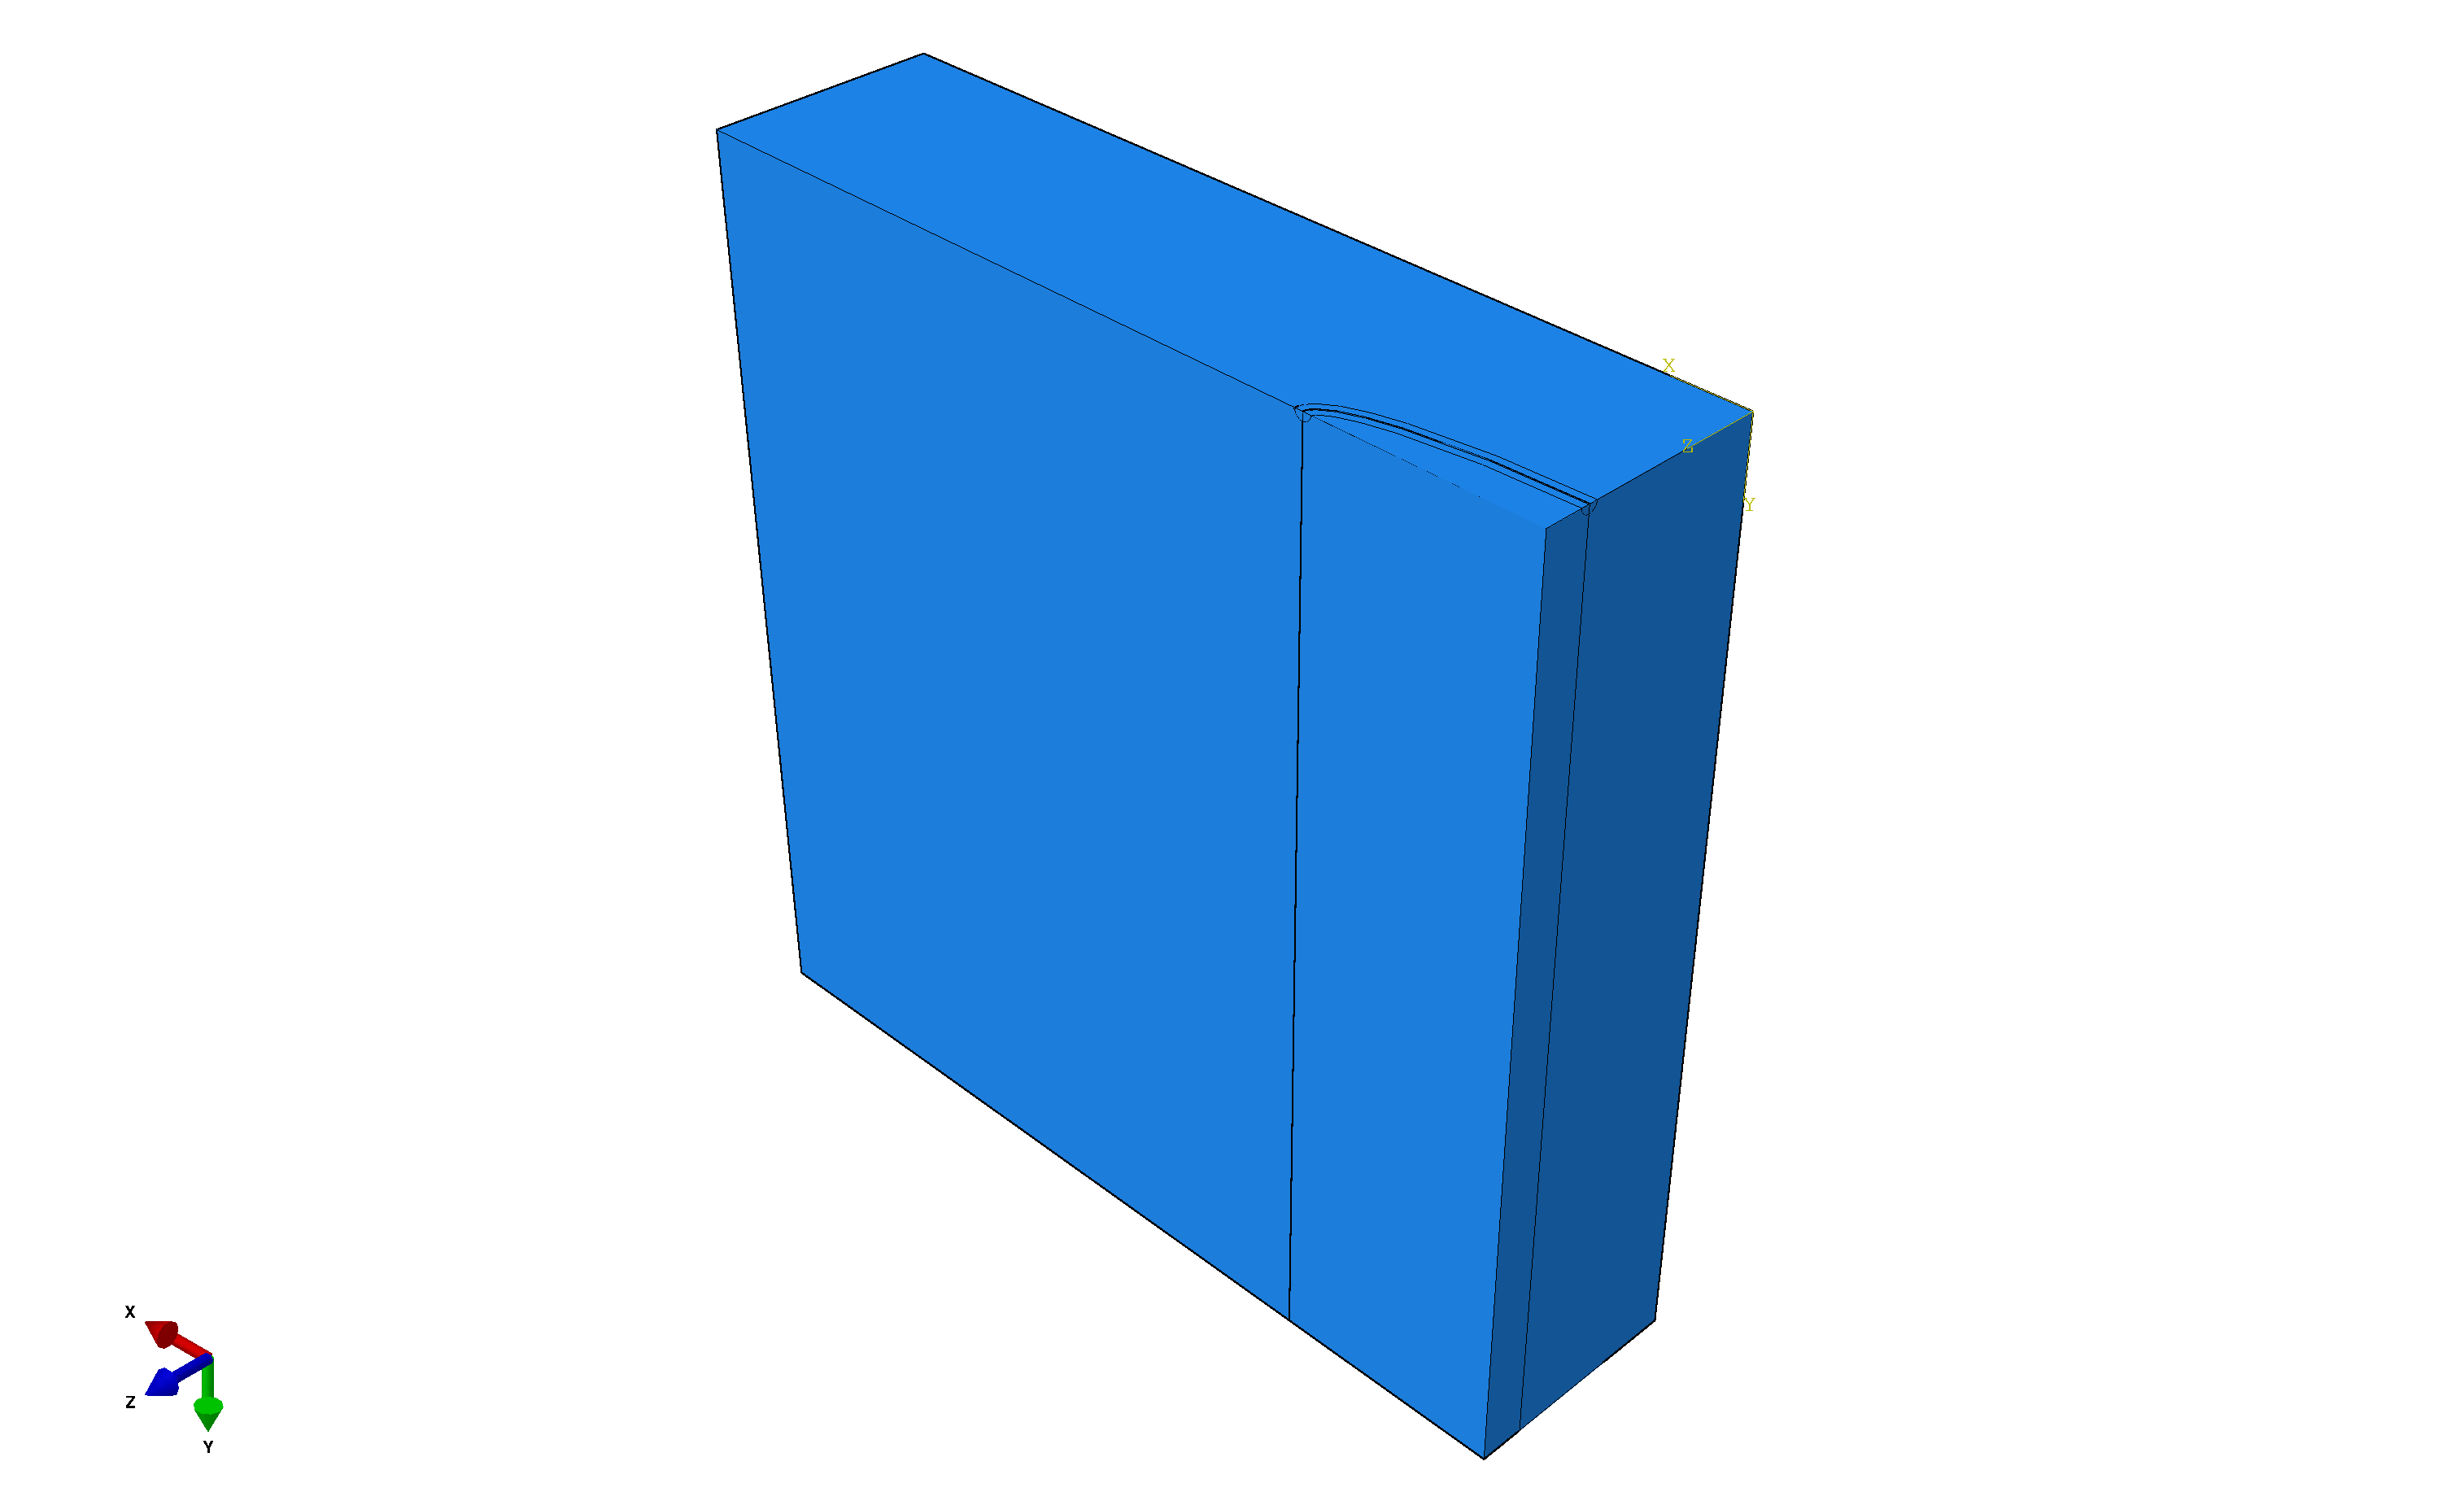
\includegraphics[width=\columnwidth]{model1-assembly}}
%    \mode<presentation>{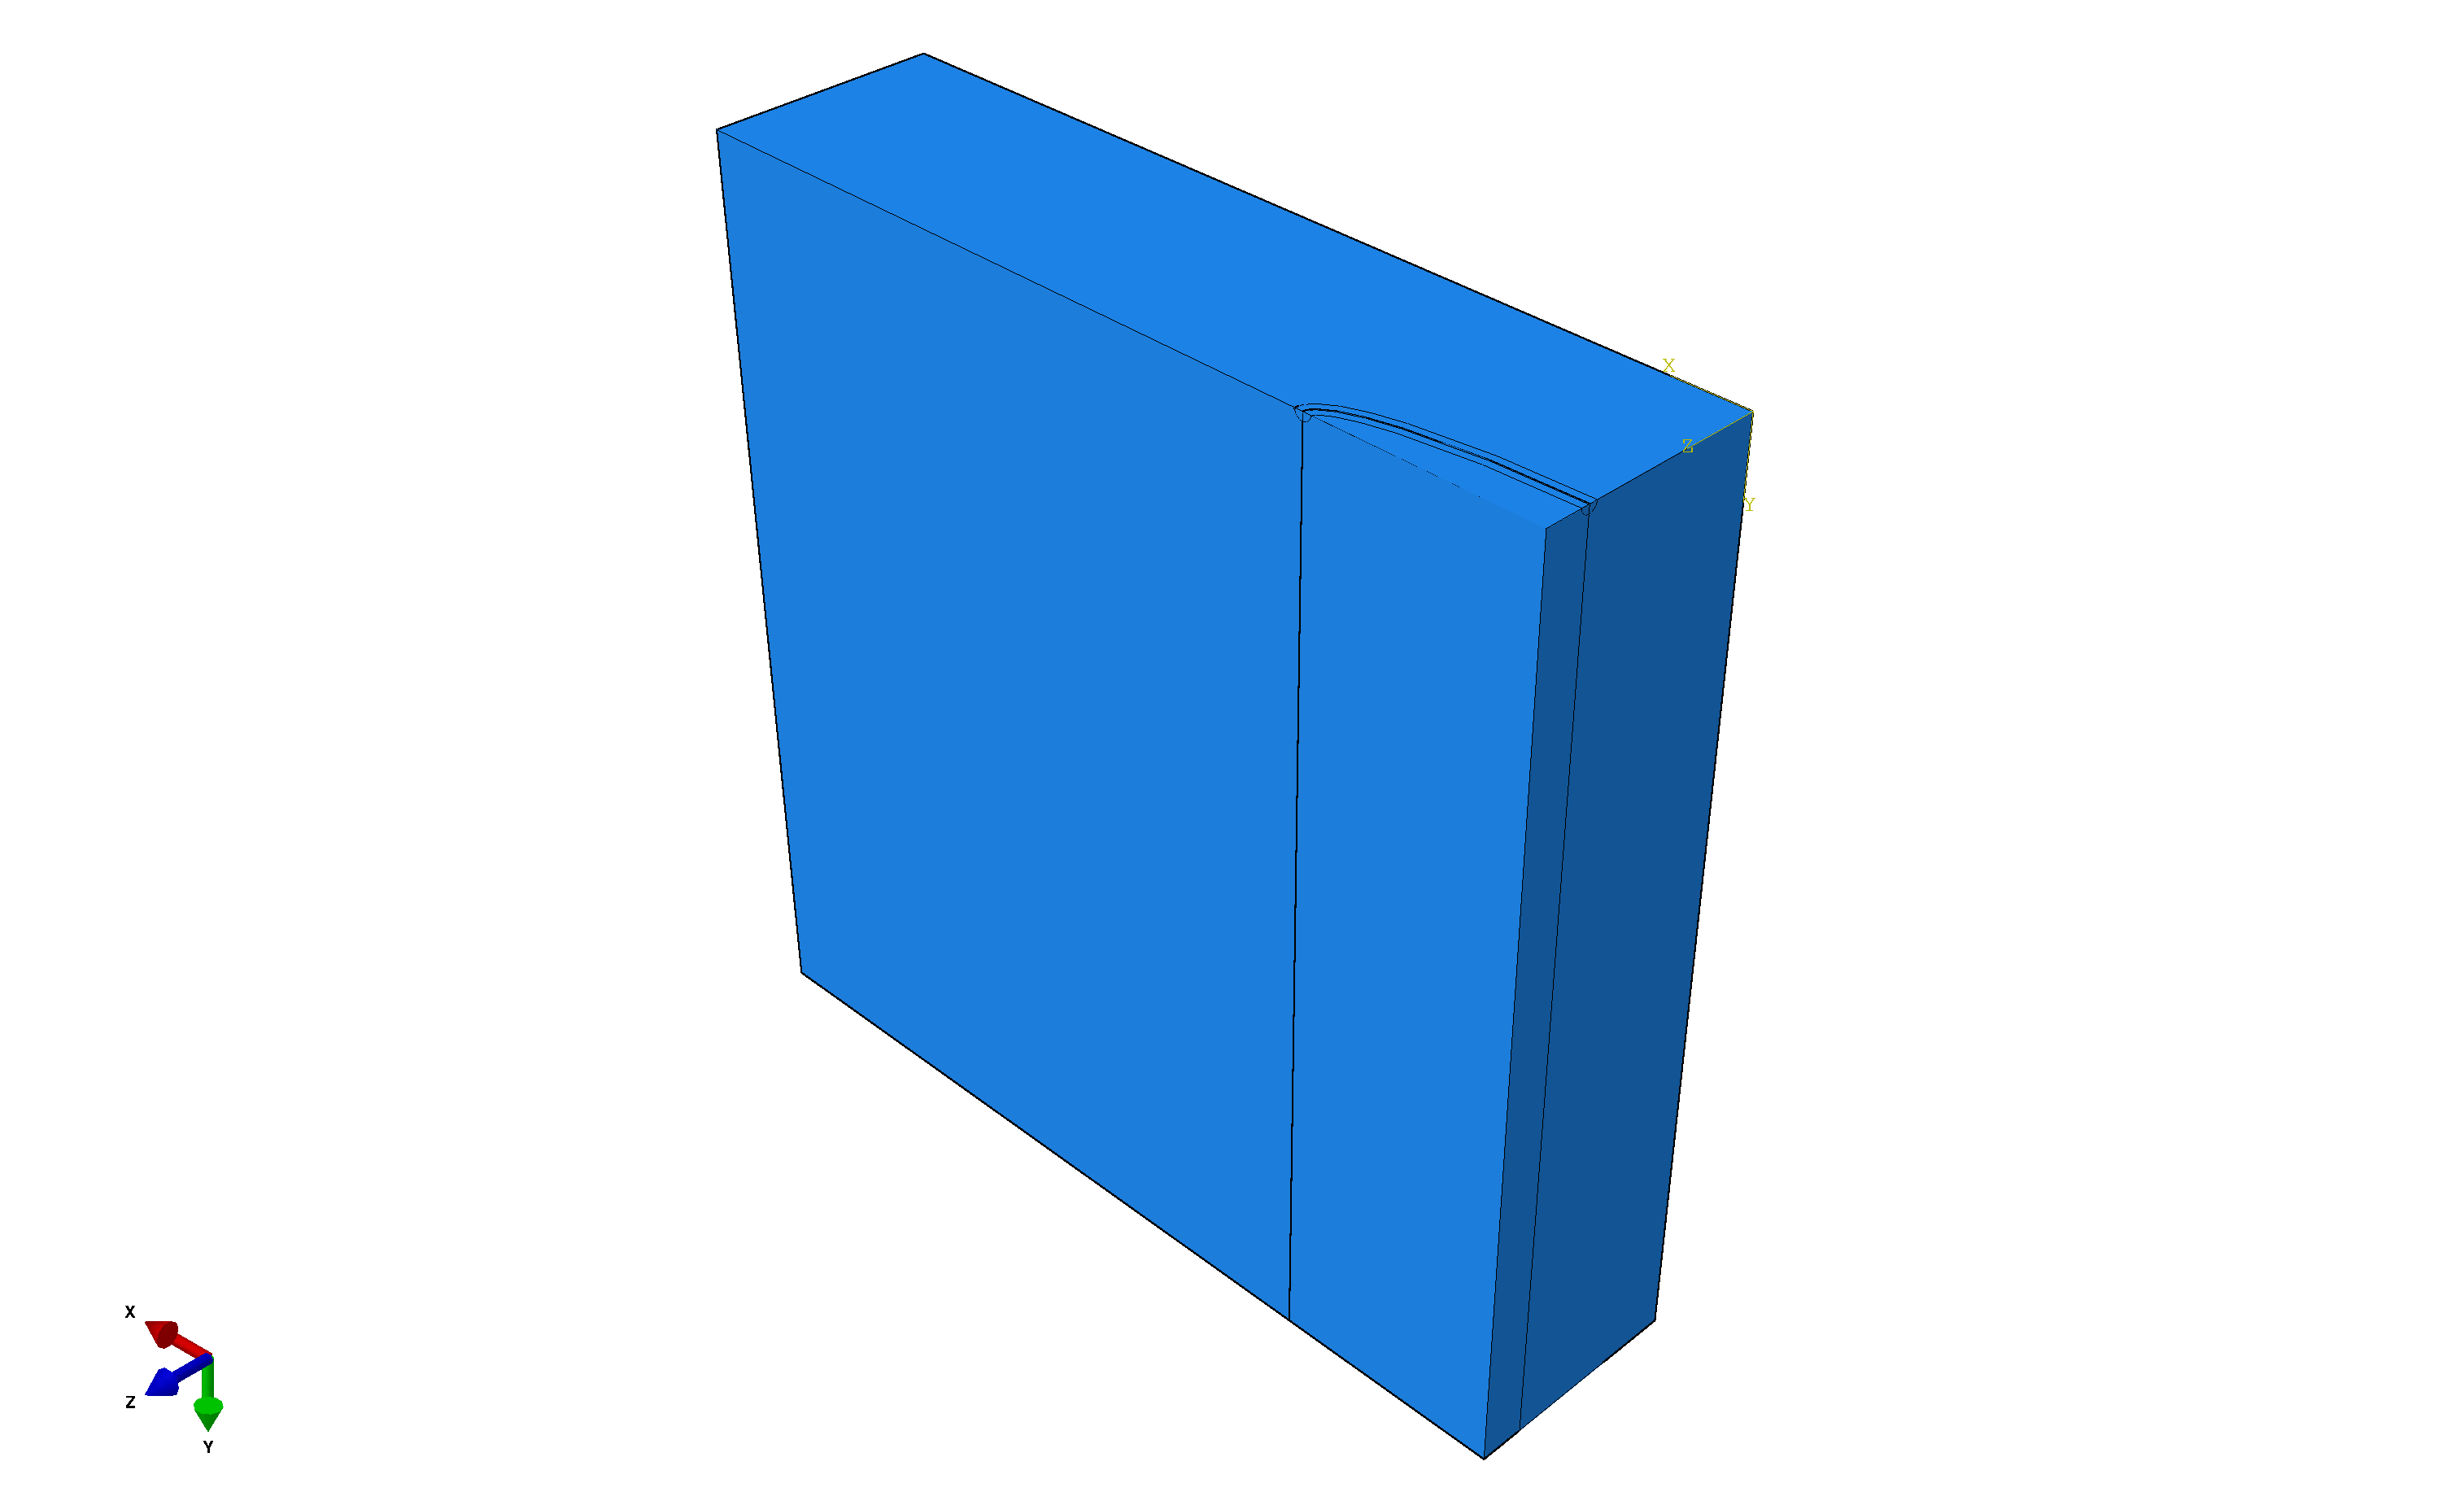
\includegraphics[width=0.7\columnwidth]{model1-assembly}}
%    \caption{McClung et al. model 1\label{fig:model1-assembly}}
%  \end{figure}
%\end{frame} \note{Model 1 is a very shallow, highly elliptical crack.}
%\begin{frame}
%  \begin{figure}
%    \centering
%    \mode<article>{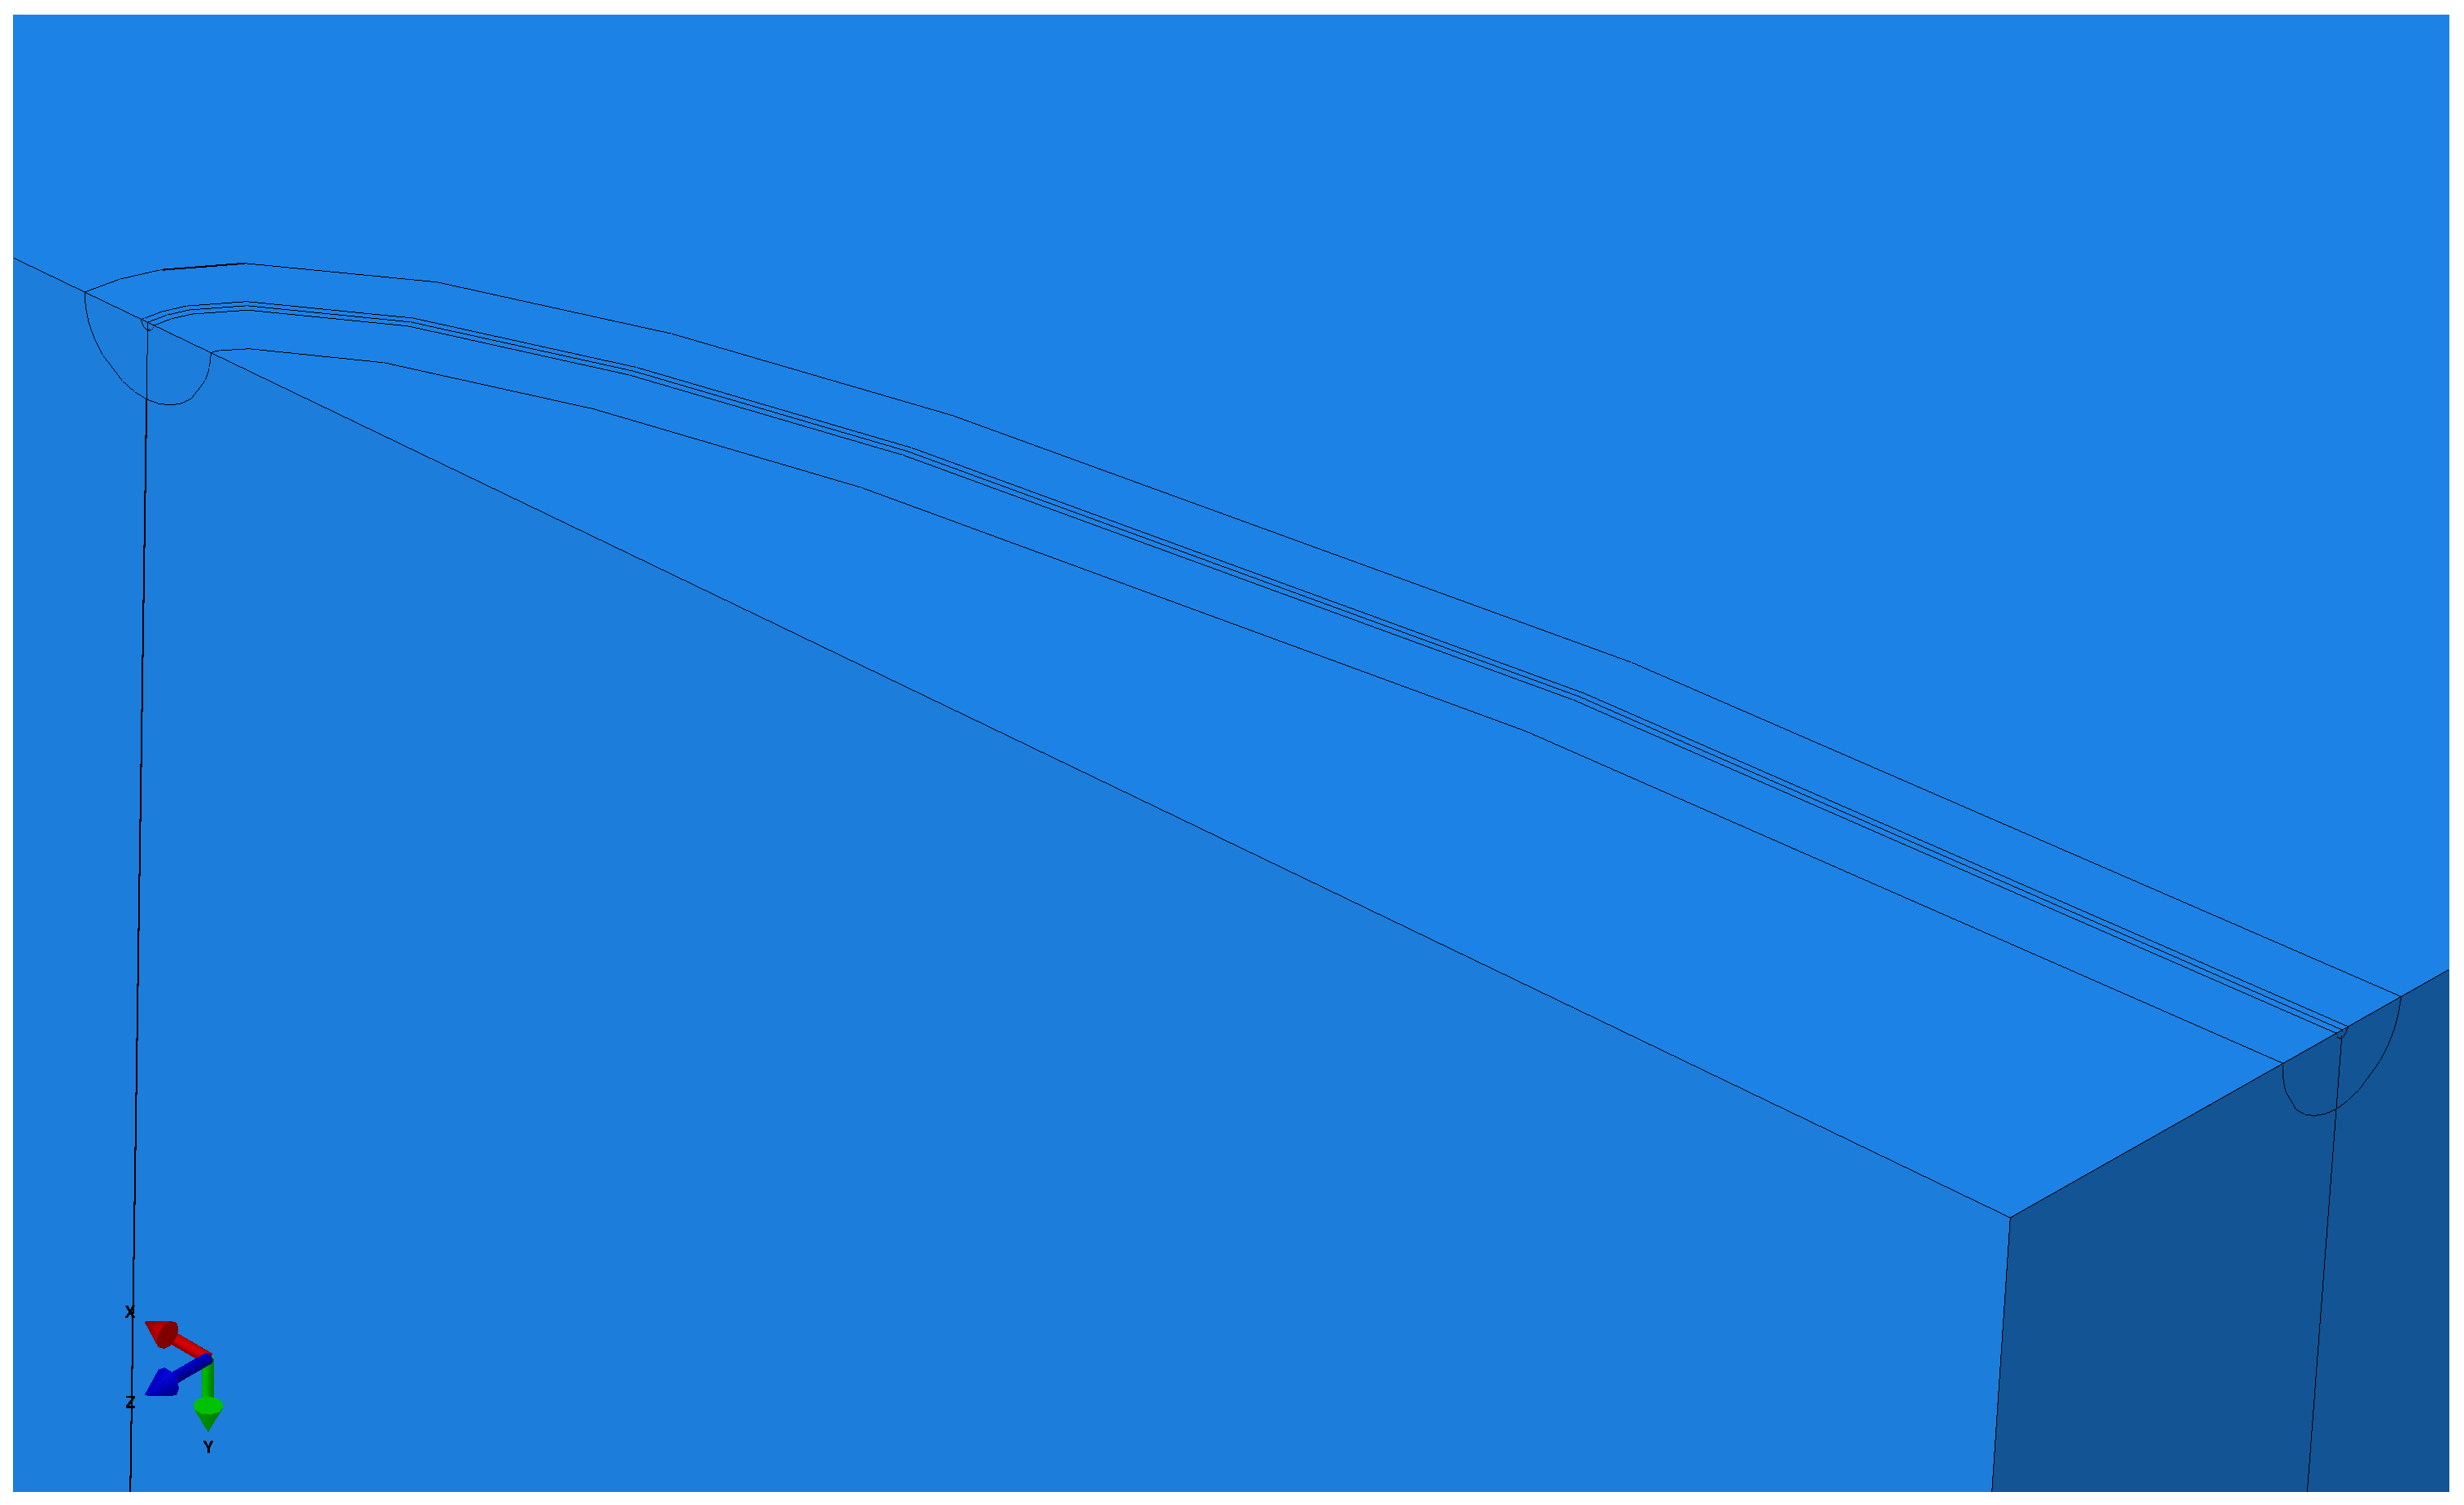
\includegraphics[width=\columnwidth]{model1-assembly-zoomed}}
%    \mode<presentation>{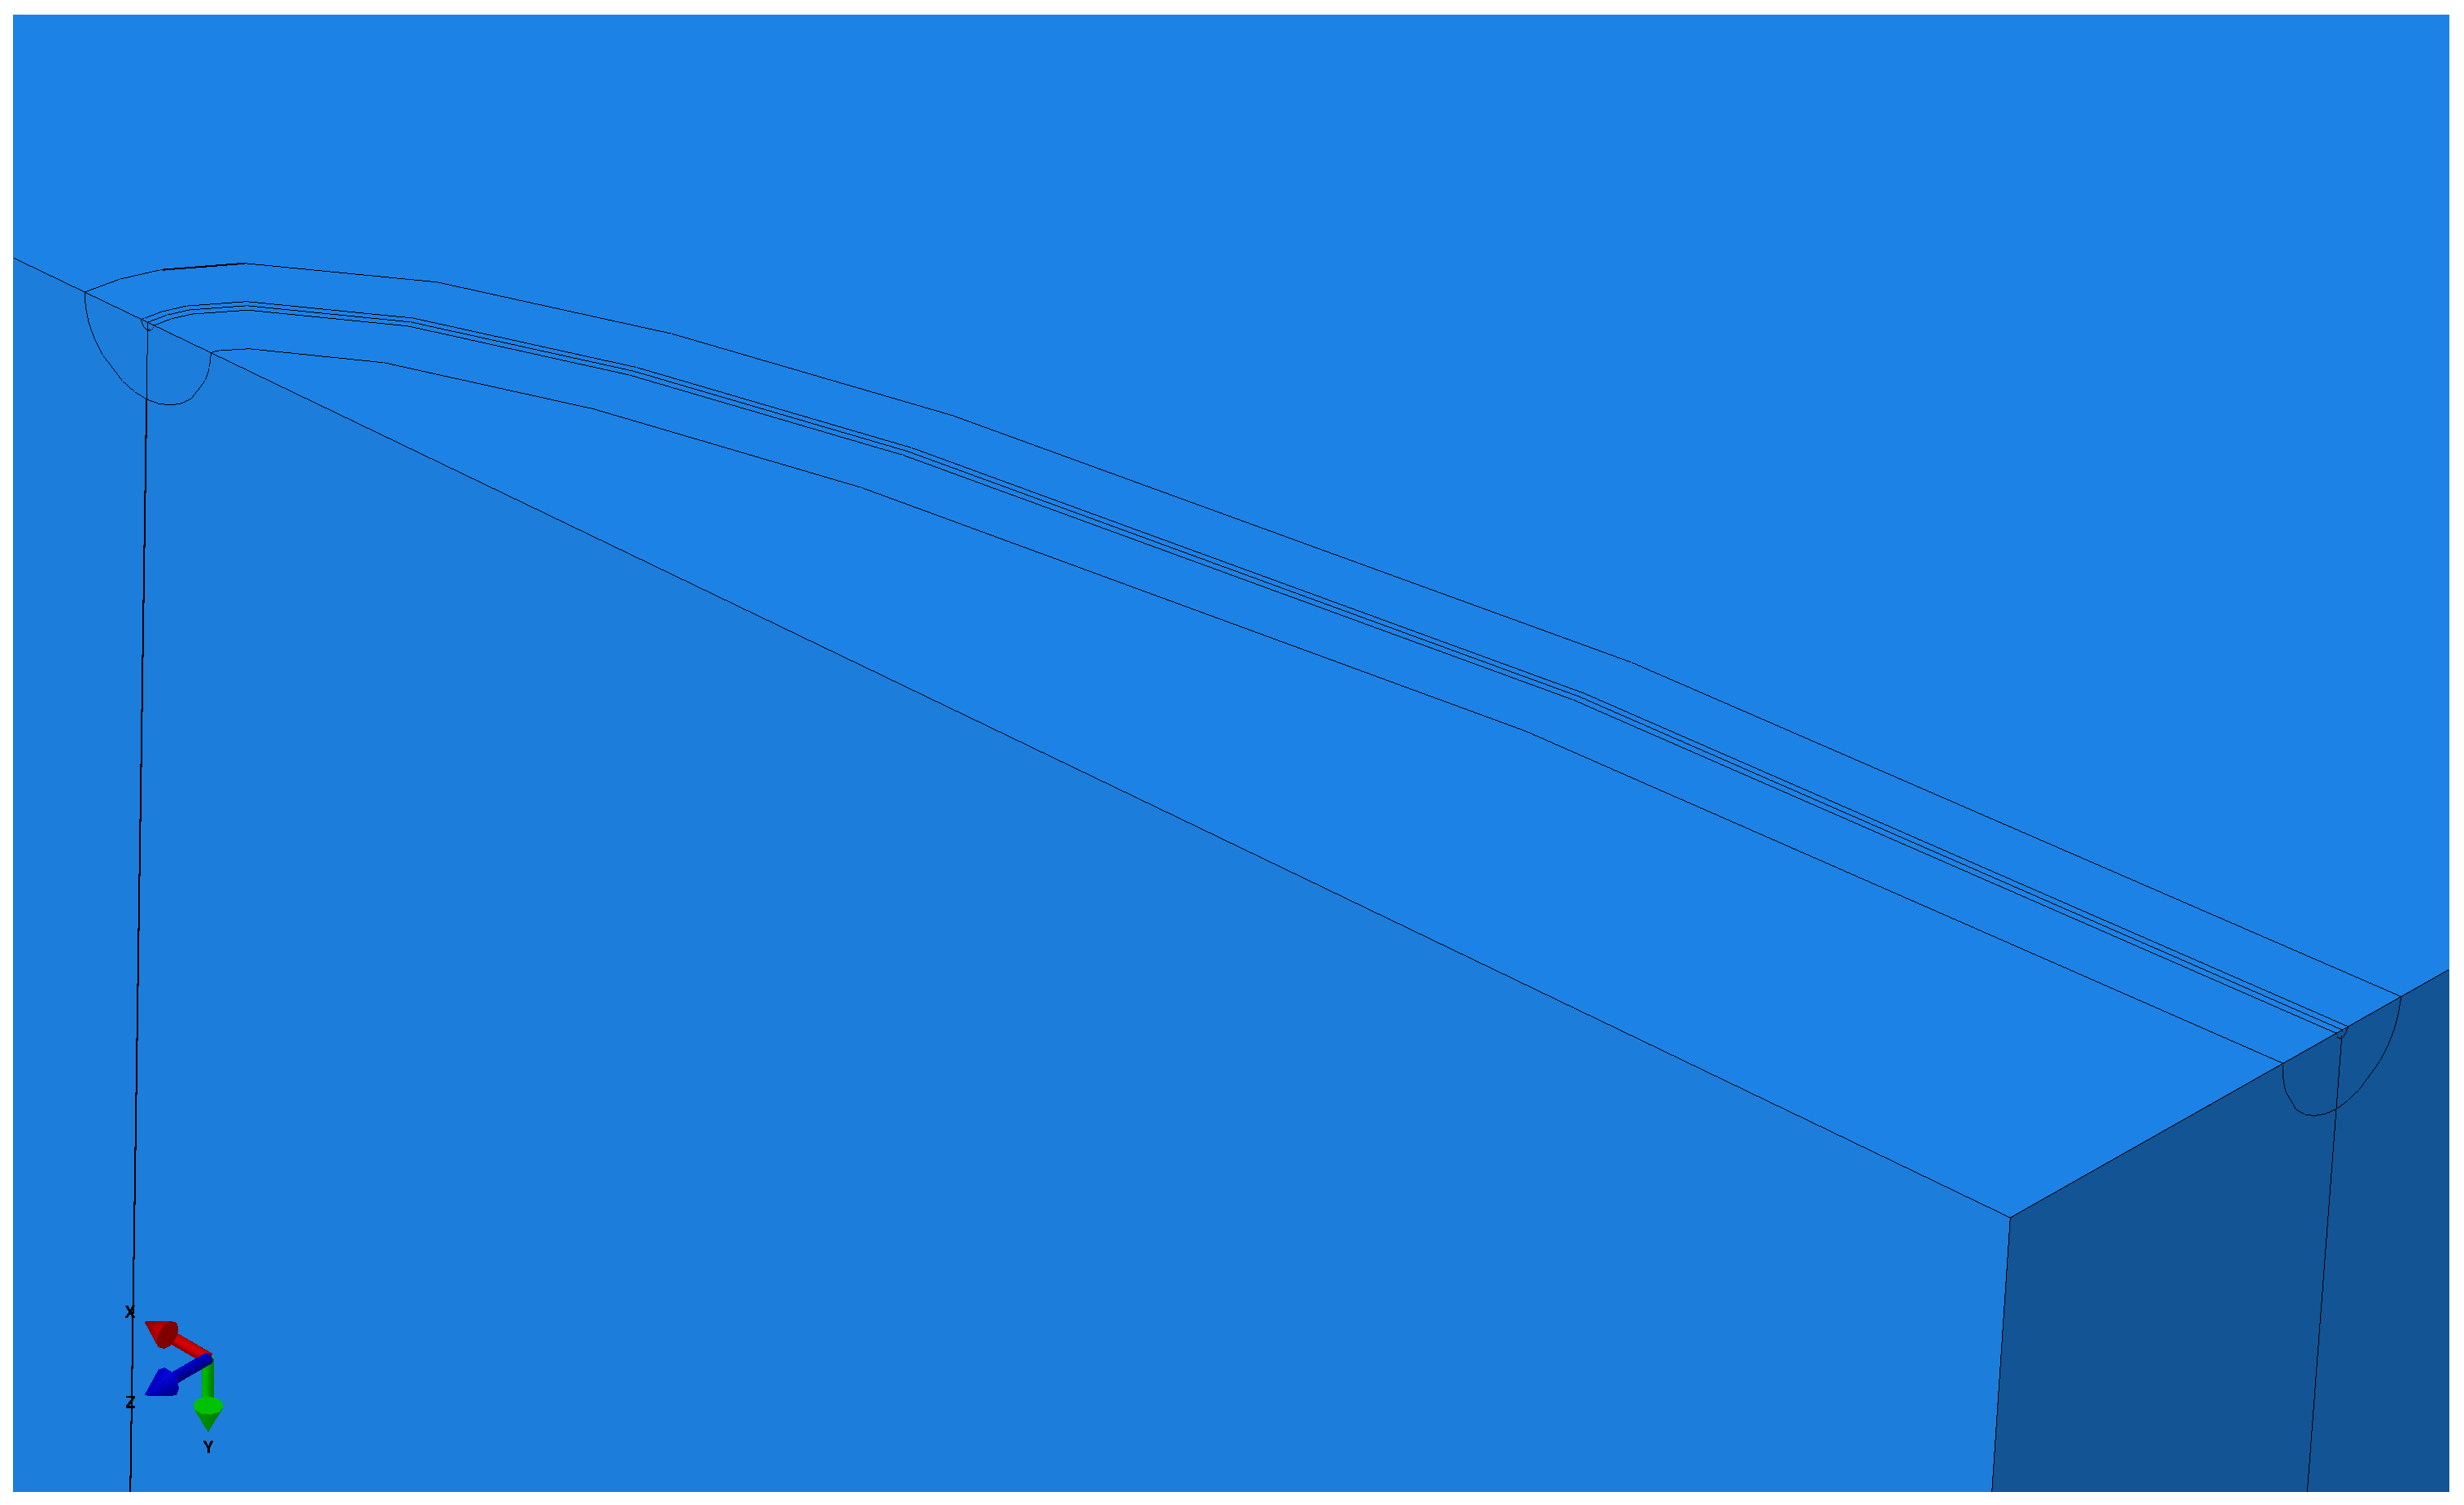
\includegraphics[width=0.7\columnwidth]{model1-assembly-zoomed}}
%    \caption{McClung et al. model 1 crack front detail\label{fig:model1-assembly-zoomed}}
%  \end{figure}
%\end{frame} \note{Zooming in on the crack front, you can see the creation of concentric regions for the crack tip and surrounding material.}
%\begin{frame}
%  \begin{figure}
%    \centering
%    \mode<article>{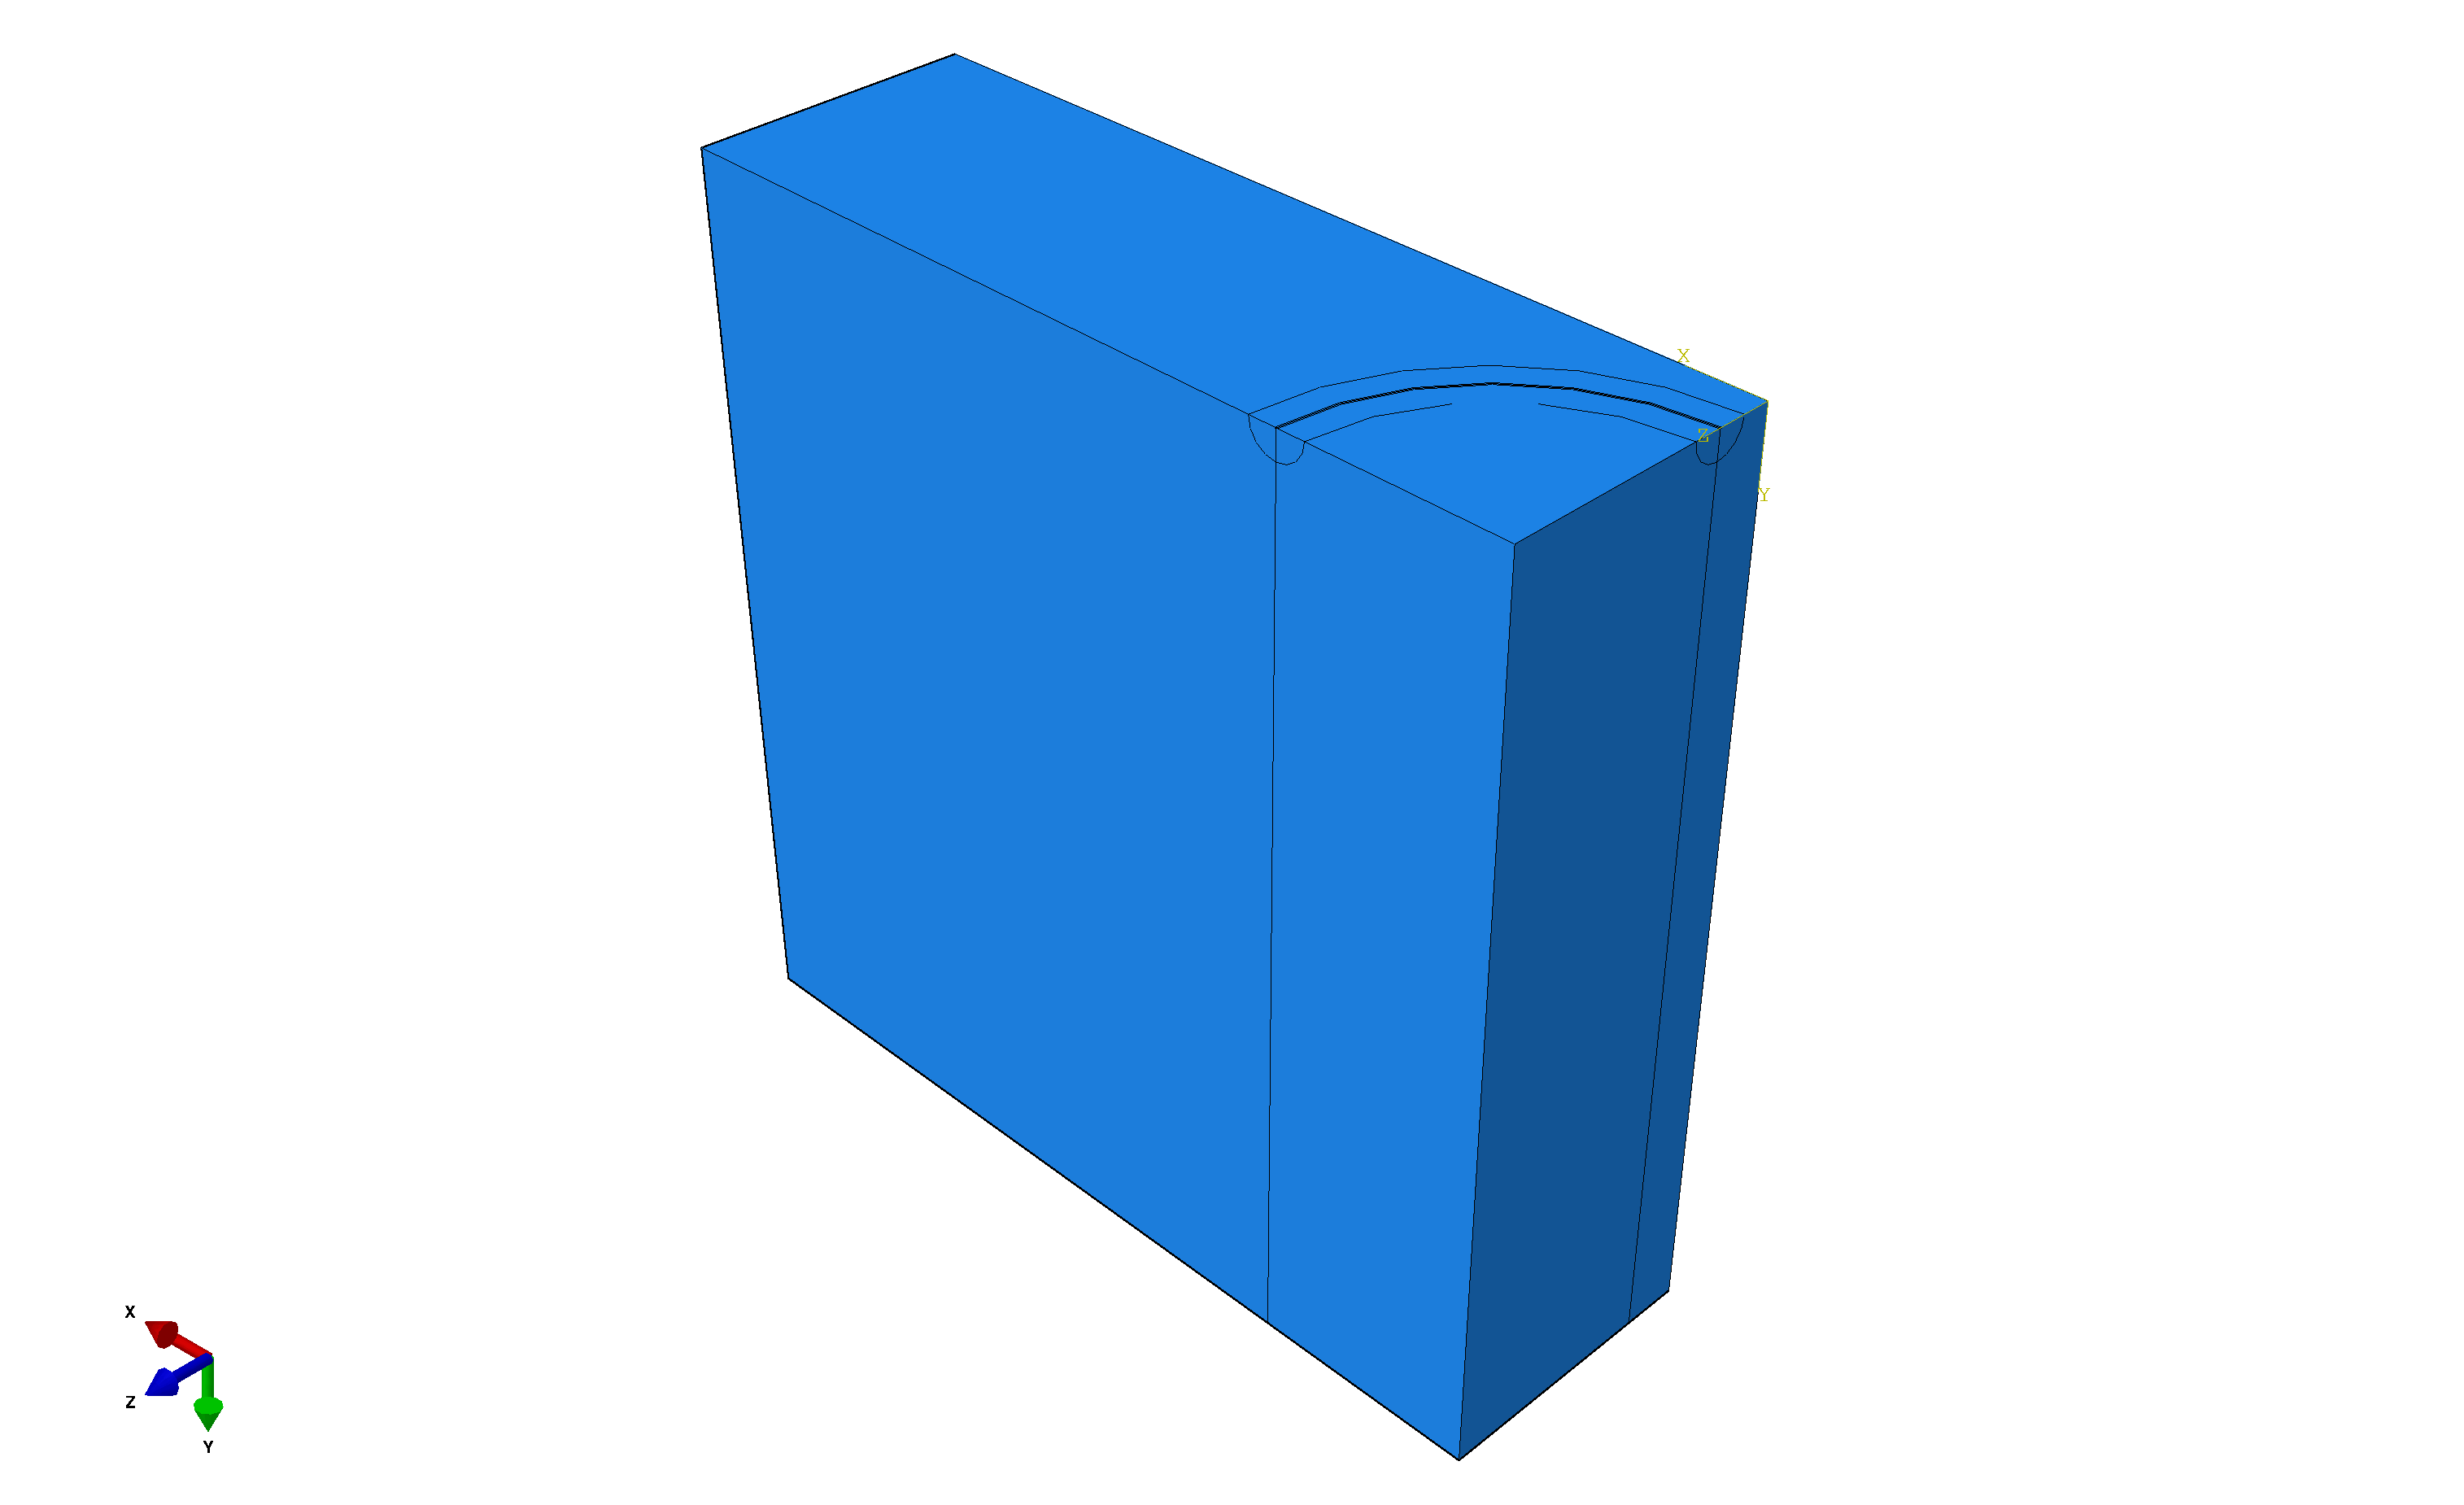
\includegraphics[width=\columnwidth]{model9-assembly}}
%    \mode<presentation>{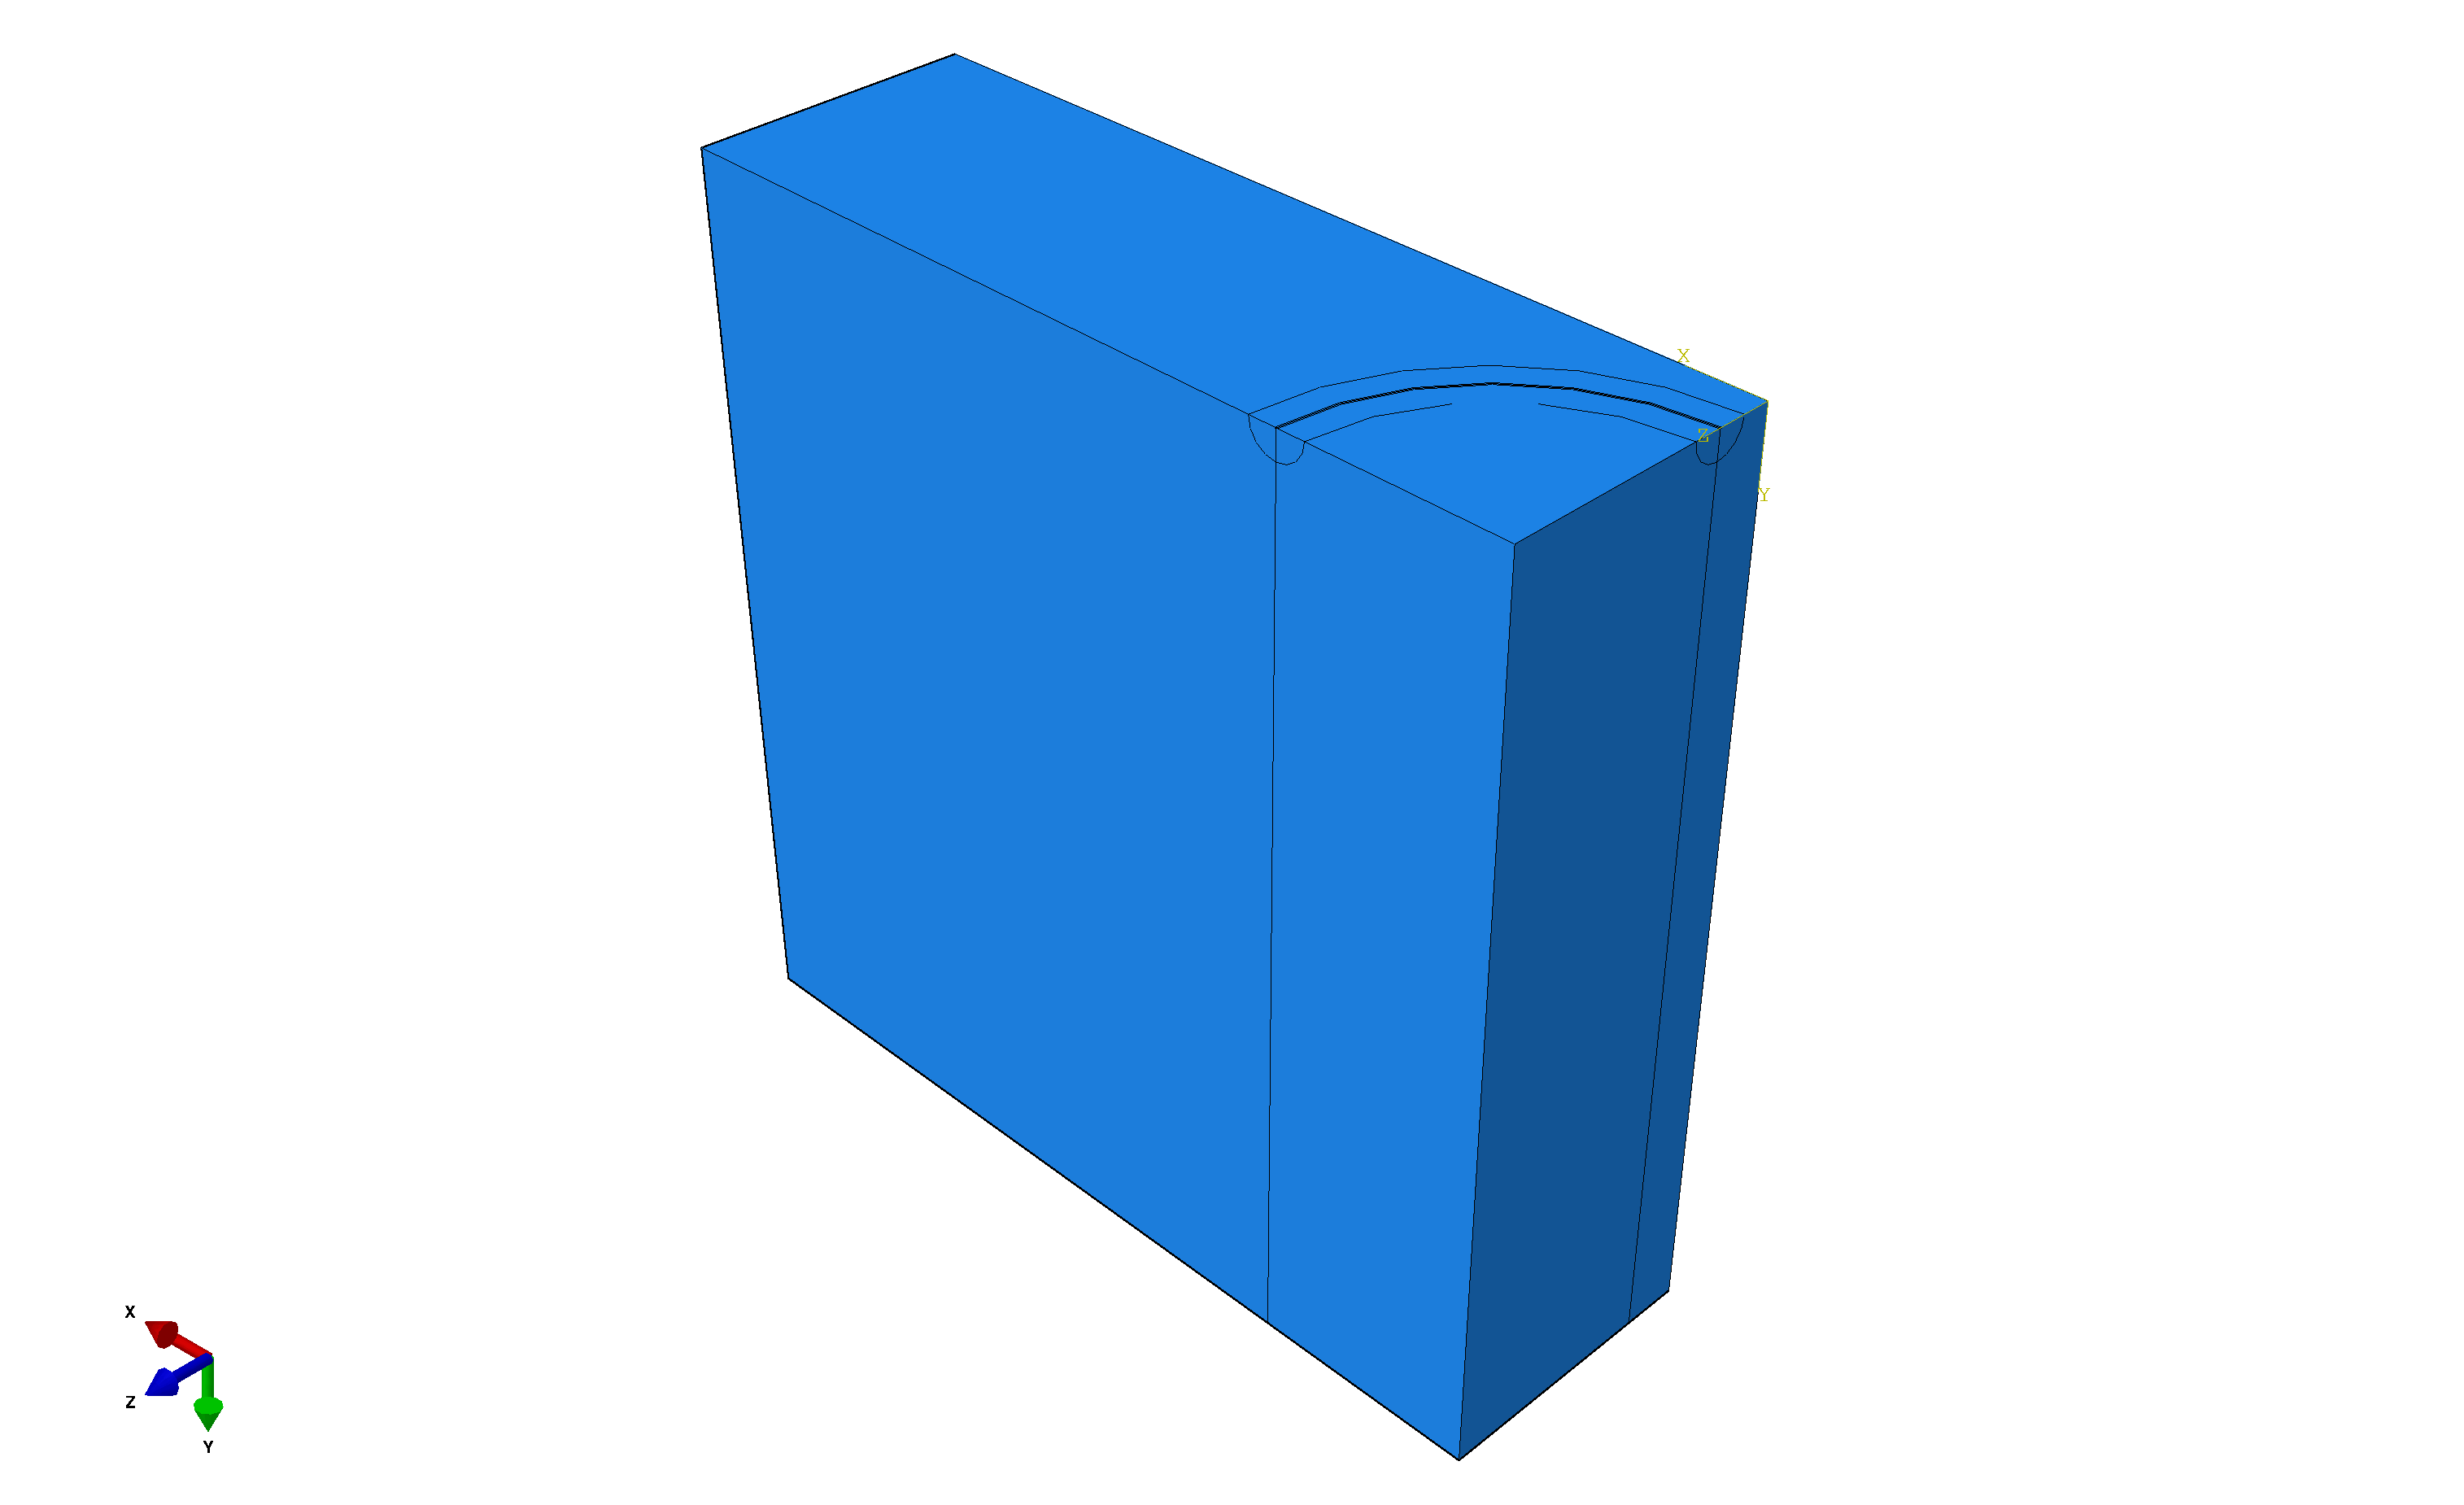
\includegraphics[width=0.7\columnwidth]{model9-assembly}}
%    \caption{McClung et al. model 9\label{fig:model9-assembly}}
%  \end{figure}
%\end{frame}
%\note{And this is Model 9, with a very deep, semi-circular crack front, generated from the same program.}
%
%\section{Further Updates to Quillen Abaqus Models}
%
\clearpage
Building from \citet{renfro2009}, the previously-described Python program created sets of models matching the plate and crack geometries given in \Cref{fig:geometries}.
For each of the nine geometries, finite element models with varying numbers of elements were created.
For each finite element mesh, one linear elastic and three Ramberg-Osgood elastic-plastic models were analyzed, and \J values were stored in the Abaqus ODB.
Finally, \hone values were calculated from the \J values to test for convergence and verification against earlier models.
A total of 144 models were analyzed, including 36 elastic models (nine geometries by four mesh densities) and 108 elastic-plastic models (nine geometries by four mesh densities by three Ramberg-Osgood hardening exponents).
Solving all the models required approximately 43 hours on one quad-core AMD Opteron compute cluster node, and created \SI{103}{\giga\byte} of output data. Extracting \hone data from the ODB files took only 7 minutes.
Mesh convergence for one model is shown in \Cref{fig:mesh-convergence}, and convergence on the ratio of \Jpl:\Jel is shown in \Cref{fig:j-convergence}.
Note that the mesh convergence is not due simply to creating smaller elements along the crack front.
As shown in \Cref{fig:model1-3-meshes}, the number of elements along the crack front only increases from 21 to 25.
Adding additional elements outside the crack region has an effect on the \J and \hone values calculated, indicating that this model set needs further development.
However, all three anomalous \hone results in \citet{quillen2005} have been eliminated, as shown in \Cref{fig:model1}.
The root cause of the anomalies (errors in the original files generated by FEACrack, possible unrecorded modifications to the files, bugs corrected in Abaqus, etc.) is still unknown.
\begin{frame}
\mode<presentation>{\begin{columns}[b]\begin{column}{0.45\textwidth}}
  \begin{figure}
    \centering
    \mode<article>{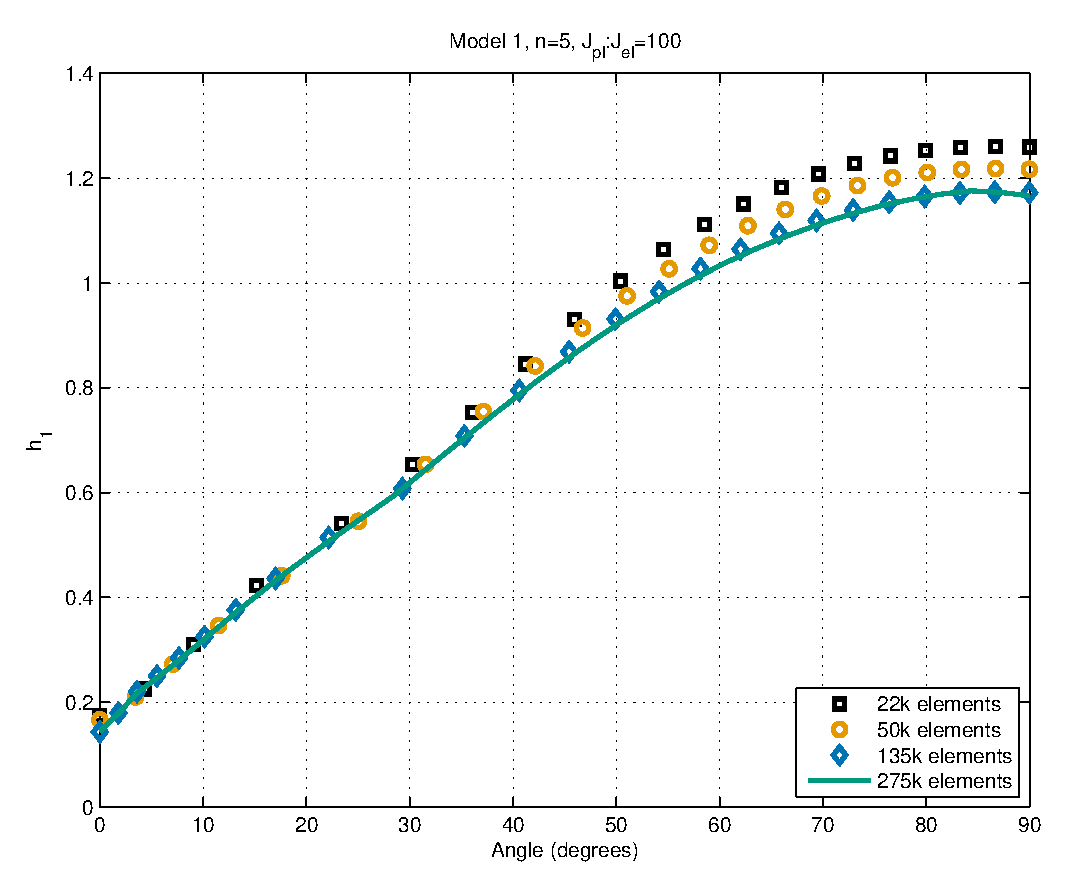
\includegraphics[width=\columnwidth]{model1_n5_mesh_convergence}}
    \mode<presentation>{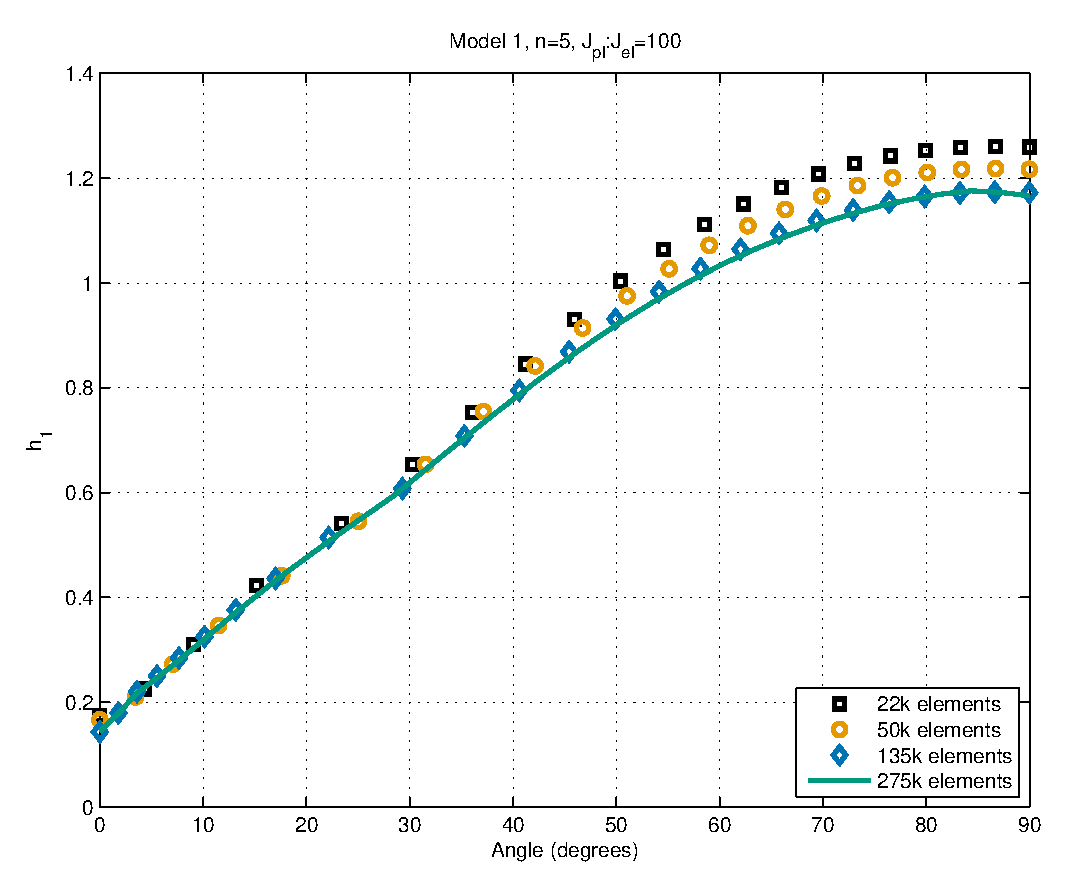
\includegraphics[width=\columnwidth]{model1_n5_mesh_convergence}}
    \caption{McClung et al. model 1 mesh convergence\label{fig:mesh-convergence}}
  \end{figure}
  \mode<presentation>{\end{column}\begin{column}{0.45\textwidth}}
%\end{frame}
%\begin{frame}
  \begin{figure}
    \centering
    \mode<article>{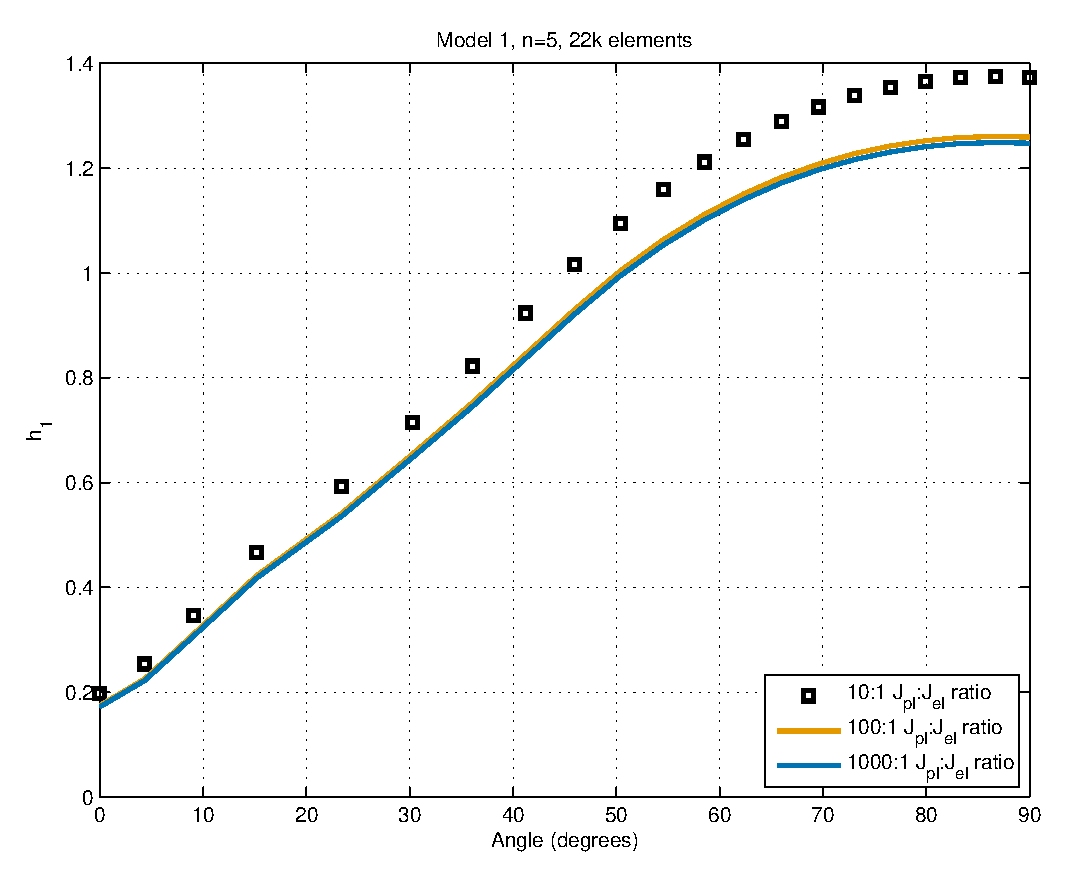
\includegraphics[width=\columnwidth]{model1_n5_J_convergence}}
    \mode<presentation>{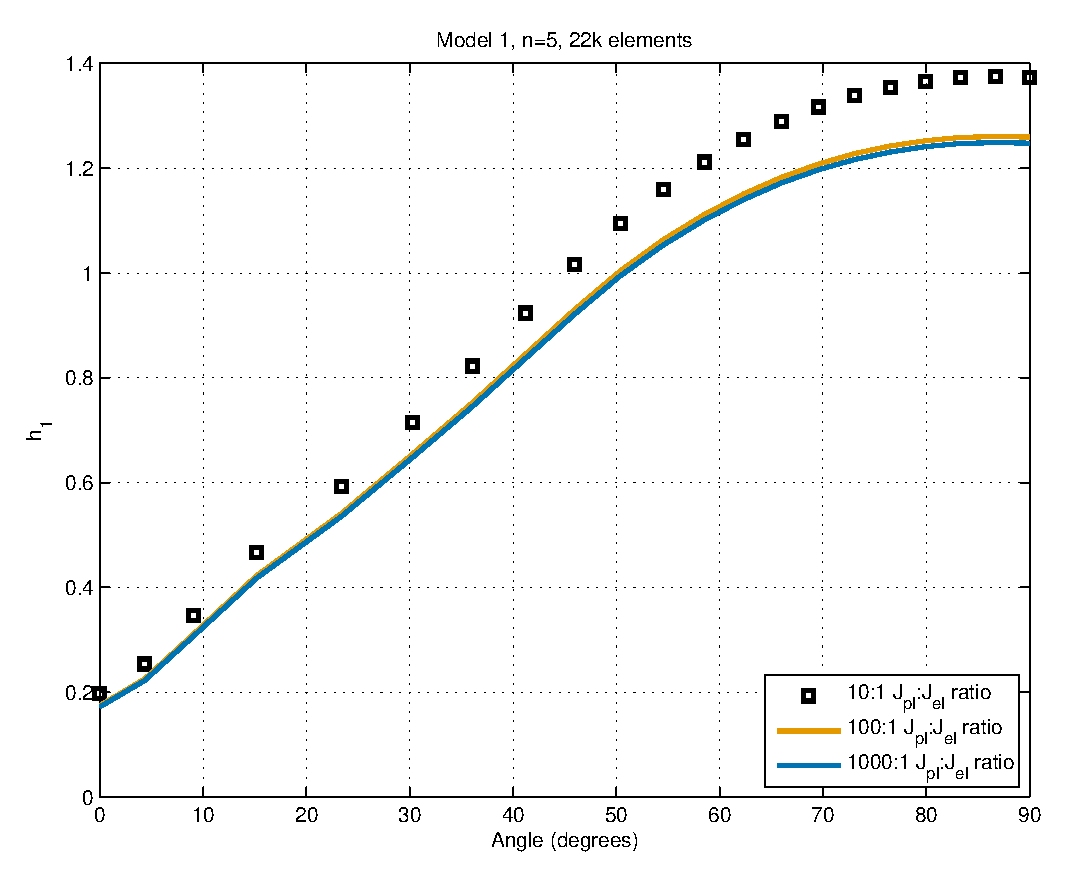
\includegraphics[width=\columnwidth]{model1_n5_J_convergence}}
    \caption{McClung et al. model 1 \J ratio convergence\label{fig:j-convergence}}
  \end{figure}
    \mode<presentation>{\end{column}\end{columns}}
\end{frame} \note{Two convergence studies were done on Model 1.

\vfill

One was to determine the influence of mesh density on \J results.

\vfill

The other was to determine the how much plastic deformation was required to give converged \J values.

\vfill

By default, when Abaqus is doing a fully plastic analysis for \J, is applies load until the ratio of \Jpl to \Jel is 10:1.

\vfill

But moving from a 10:1 ratio to a 100:1 ratio yielded substantial \J and \hone differences deep in the crack.

\vfill

The 100:1 and 1000:1 ratios returned virtually identical results.

\vfill
}
\begin{frame}
\mode<presentation>{\begin{columns}[t]\begin{column}{0.45\textwidth}}
  \begin{figure}
    \centering
    \mode<article>{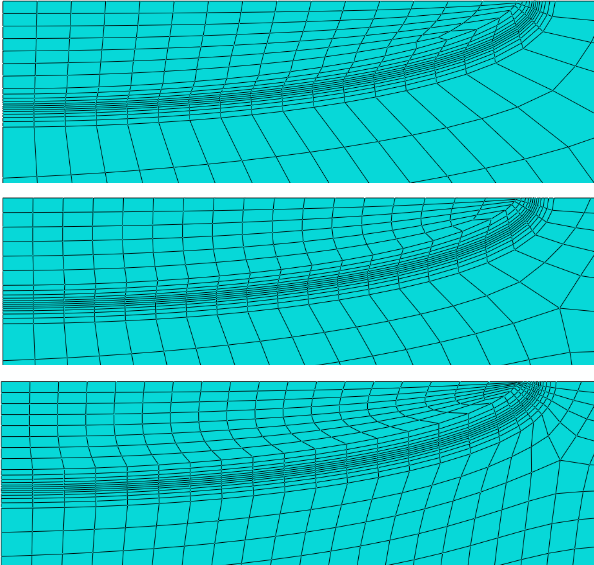
\includegraphics[width=\columnwidth]{model1-3-meshes}}
    \mode<presentation>{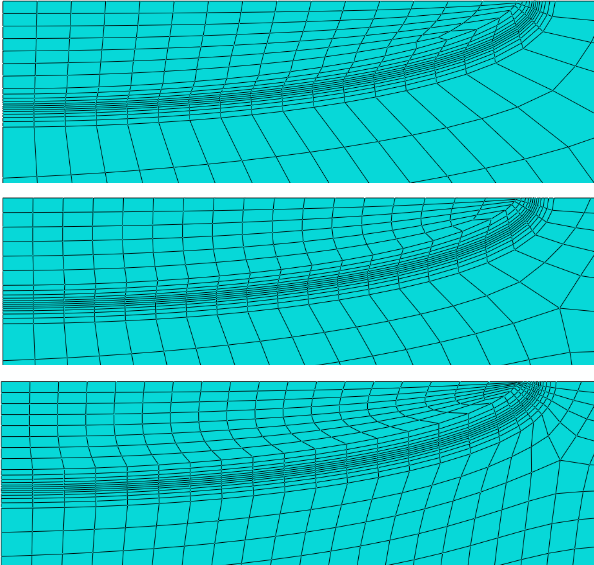
\includegraphics[width=0.8\columnwidth]{model1-3-meshes}}
    \caption{McClung et al. model 1 crack front mesh detail\label{fig:model1-3-meshes}}
  \end{figure}
  \mode<presentation>{\end{column}\begin{column}{0.45\textwidth}}
%\end{frame}
%
%\newcommand{\hfigure}[1]{
%\begin{figure} \centering \includegraphics[width=\hwidth]{h1_model#1}
%\caption{\hone comparison between McClung et al., Lei, Quillen, and Renfro, model #1 \label{fig:model#1}}
%\end{figure}
%}
%\newcommand{\hmissingfigure}[1]{
%\begin{figure} \centering \missingfigure[figwidth=\hwidth]{model #1}
%\caption{\hone comparison between McClung et al., Lei, Quillen, and Renfro, model #1 \label{fig:model#1}}
%\end{figure}
%}
%
%\begin{frame}
%  \mode<presentation>{
%    \frametitle{\hone comparisons among McClung et al., Lei, and Renfro, model 1}
%  }
  \begin{figure}
    \centering
    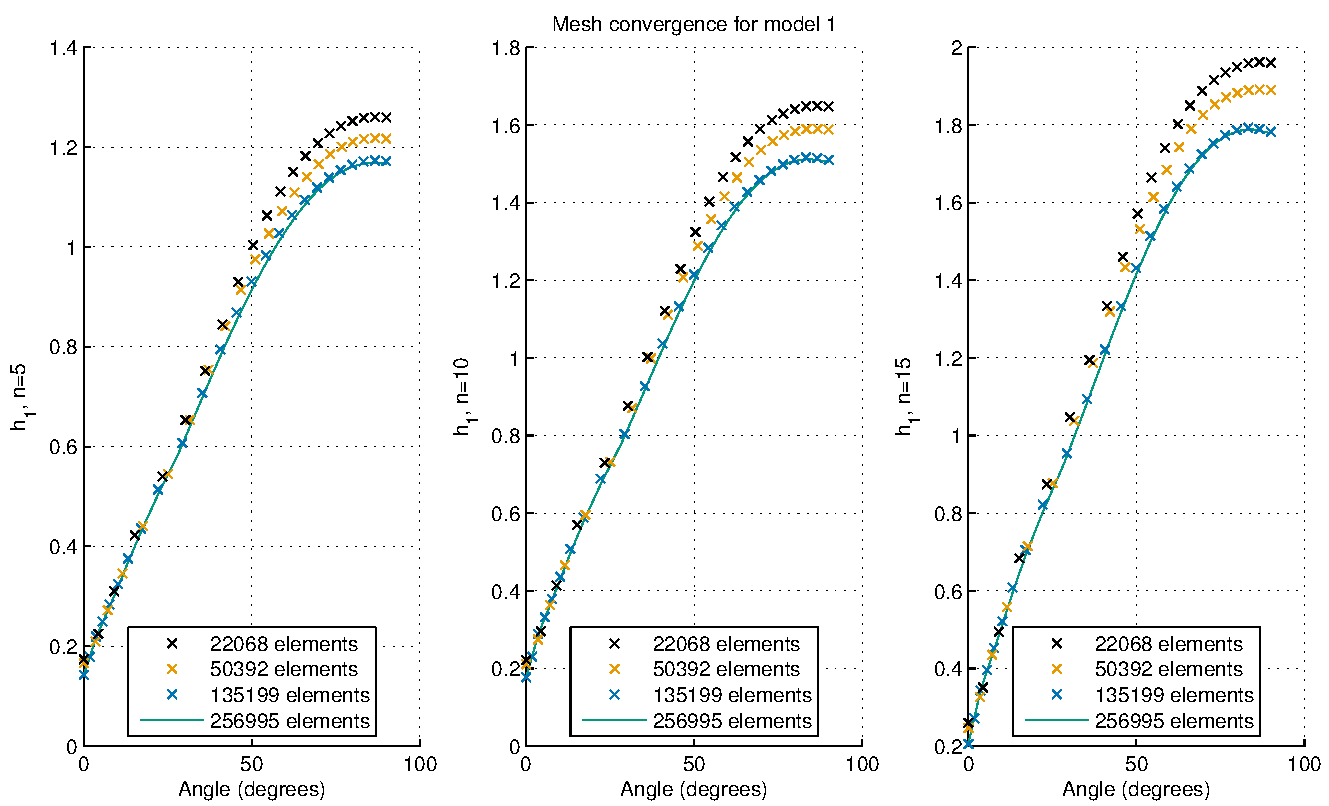
\includegraphics[width=\columnwidth]{h1_model1}
    \mode<article>{\caption{\hone comparison between McClung et al., Lei, and Renfro, model 1 \label{fig:model1}}}
  \end{figure}
    \mode<presentation>{\end{column}\end{columns}}
\end{frame}
\note{Looking at the effect of the Ramberg-Osgood hardening exponent, it appears that harder materials (higher \(n\)) show more deviations from the McClung and Lei results than the softer material.}
